\documentclass[hyperref=colorlinks]{beamer}
\mode<presentation>
\usetheme{iclpt}
\setbeamertemplate{navigation symbols}{}
\setbeamertemplate{headline}{
\begin{beamercolorbox}[leftskip=.2cm,rightskip=.2cm,topskip=.2cm,ht=1.1cm,dp=0.1cm,wd=\textwidth]{institute in head/foot}
  
\includegraphics[height=1cm]{icl.pdf}
  \hfill
  
\includegraphics[height=1cm]{../Pics/CMS-Color.pdf}
\end{beamercolorbox}
}
\setbeamertemplate{footline}{
\begin{beamercolorbox}[ht=.55cm,dp=0.4cm,wd=\textwidth,leftskip=.3cm]{author in head/foot}%
  \begin{minipage}[c]{5cm}%
    \usebeamerfont{author in head/foot}
    \insertshortauthor 
    \insertshorttitle
    \end{minipage}\hfill%
  \insertframenumber{} / \pageref{lastframe}
  \hfill
  \begin{minipage}{6cm}
    \hfill
  \end{minipage}
\end{beamercolorbox}%
}

\usepackage{color}
\usepackage{tabularx,colortbl}
\usepackage{graphicx}
\usepackage{pdfpages}
\usepackage{feynmp}
\usepackage{tikz}
\usetikzlibrary{calc, shapes, backgrounds,arrows,positioning}
\DeclareGraphicsRule{*}{mps}{*}{}

\title{\vspace{-0.2cm} VBF Higgs to Invisible}
\subtitle{\vspace{-0.7cm}}
\author[]{}%\underline{P. Dunne}} % A.M. Magnan and A. Nikitenko Joao Pela with \\ R. Aggleton, J. Brooke: Bristol \\ C.Asawangtrakuldee, Q.Li: Peking \\ P. Srimanobhas: Chulalongkorn \\ S. Kumar, K. Mazumdar: Mumbai}
\titlegraphic{
  \vspace{-0.7cm}
  %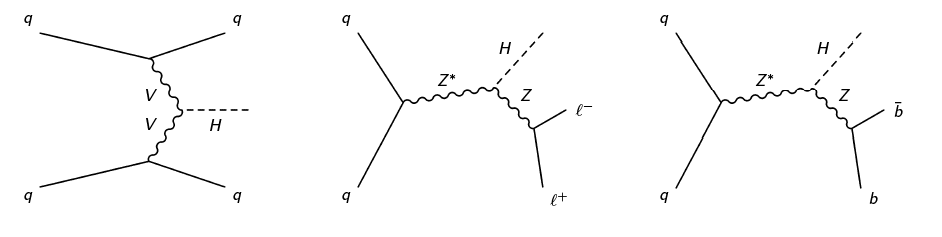
\includegraphics[width=\textwidth]{TalkPics/invcomb021213/feyndiags}
  %% \begin{fmfgraph*}(100,70)
  %%         \fmfleft{i1,i2}
  %%         \fmfright{o1,o2,o3}
  %%         \fmf{fermion}{i1,v1,o1}
  %%         \fmf{fermion}{i2,v2,o3}
  %%         \fmf{phantom,tension=4/5}{v1,v2}
  %%         \fmffreeze
  %%         \fmf{photon,label=$W,,Z$}{v1,v3}
  %%         \fmf{photon,label=$W,,Z$}{v2,v3}
  %%         \fmf{dashes}{v3,o2}
  %%         \fmflabel{$q$}{i1}
  %%         \fmflabel{$q$}{i2}
  %%         \fmflabel{$q$}{o1}
  %%         \fmflabel{$q$}{o3}
  %%         \fmflabel{$H$}{o2}
  %%       \end{fmfgraph*}
}
\date{}
\begin{document}
\begin{fmffile}{higgsexoupdatefeyndiags}
\tikzstyle{every picture}+=[remember picture]

%TITLE PAGE
\section{Title}
\begin{frame}
  \titlepage
  
\end{frame}

\begin{frame}
  \frametitle{W \& Z MC}
  \begin{block}{Run 1 Reminder}
    \begin{itemize}
    \item In run 1 we split $W\rightarrow\ell\nu$ samples by lepton at generator level
    \item $W\rightarrow\tau\nu$ events were classified according to $\tau$ decay:
    \item[-] e.g. $W\rightarrow\tau\nu\rightarrow\mu\nu\nu\nu$ put in muon category etc.
    \item $Z\rightarrow\mu\mu$ samples split into high and low generated Z $p_{T}$
    \item All of the above done by looking at status 3 particles
    \end{itemize}
  \end{block}
  \begin{block}{Run 2}
    \begin{itemize}
    \item Phys 14 only has one Z MC sample so don't need to split
    \item W still needs splitting by lepton flavour
    \item[-] No more status 3, need a replacement
    \end{itemize}
    \end{block}
\end{frame}

\begin{frame}
  \frametitle{DY Comparison}
  \begin{block}{}
    \begin{itemize}
    \item As recommended weights now removed to make it clearer if difference is from gen/reconstruction
    \item Distributions still normalised to 1
    \item Same set of plots as for QCD and signal included for reference
    \item Selection as for QCD is: $\eta_{j1} \cdot \eta_{j2}<0,\, \eta_{j1}<4.7,\, \eta_{j2}<4.7,$
      $p_{T}^{\text{j1}}>50 \,\text{GeV},\,p_{T}^{\text{j2}}>40\,\text{GeV},$
      $\Delta\eta_{jj}>3.6,\, M_{jj}>800\,\text{GeV},$
      $MET>90\,\text{GeV},$
      $METsig>3.$
    \end{itemize}
  \end{block}
\end{frame}

\begin{frame}
  \frametitle{DY Comparison: run 1 vs run 2: Jet $p_{T}$}
  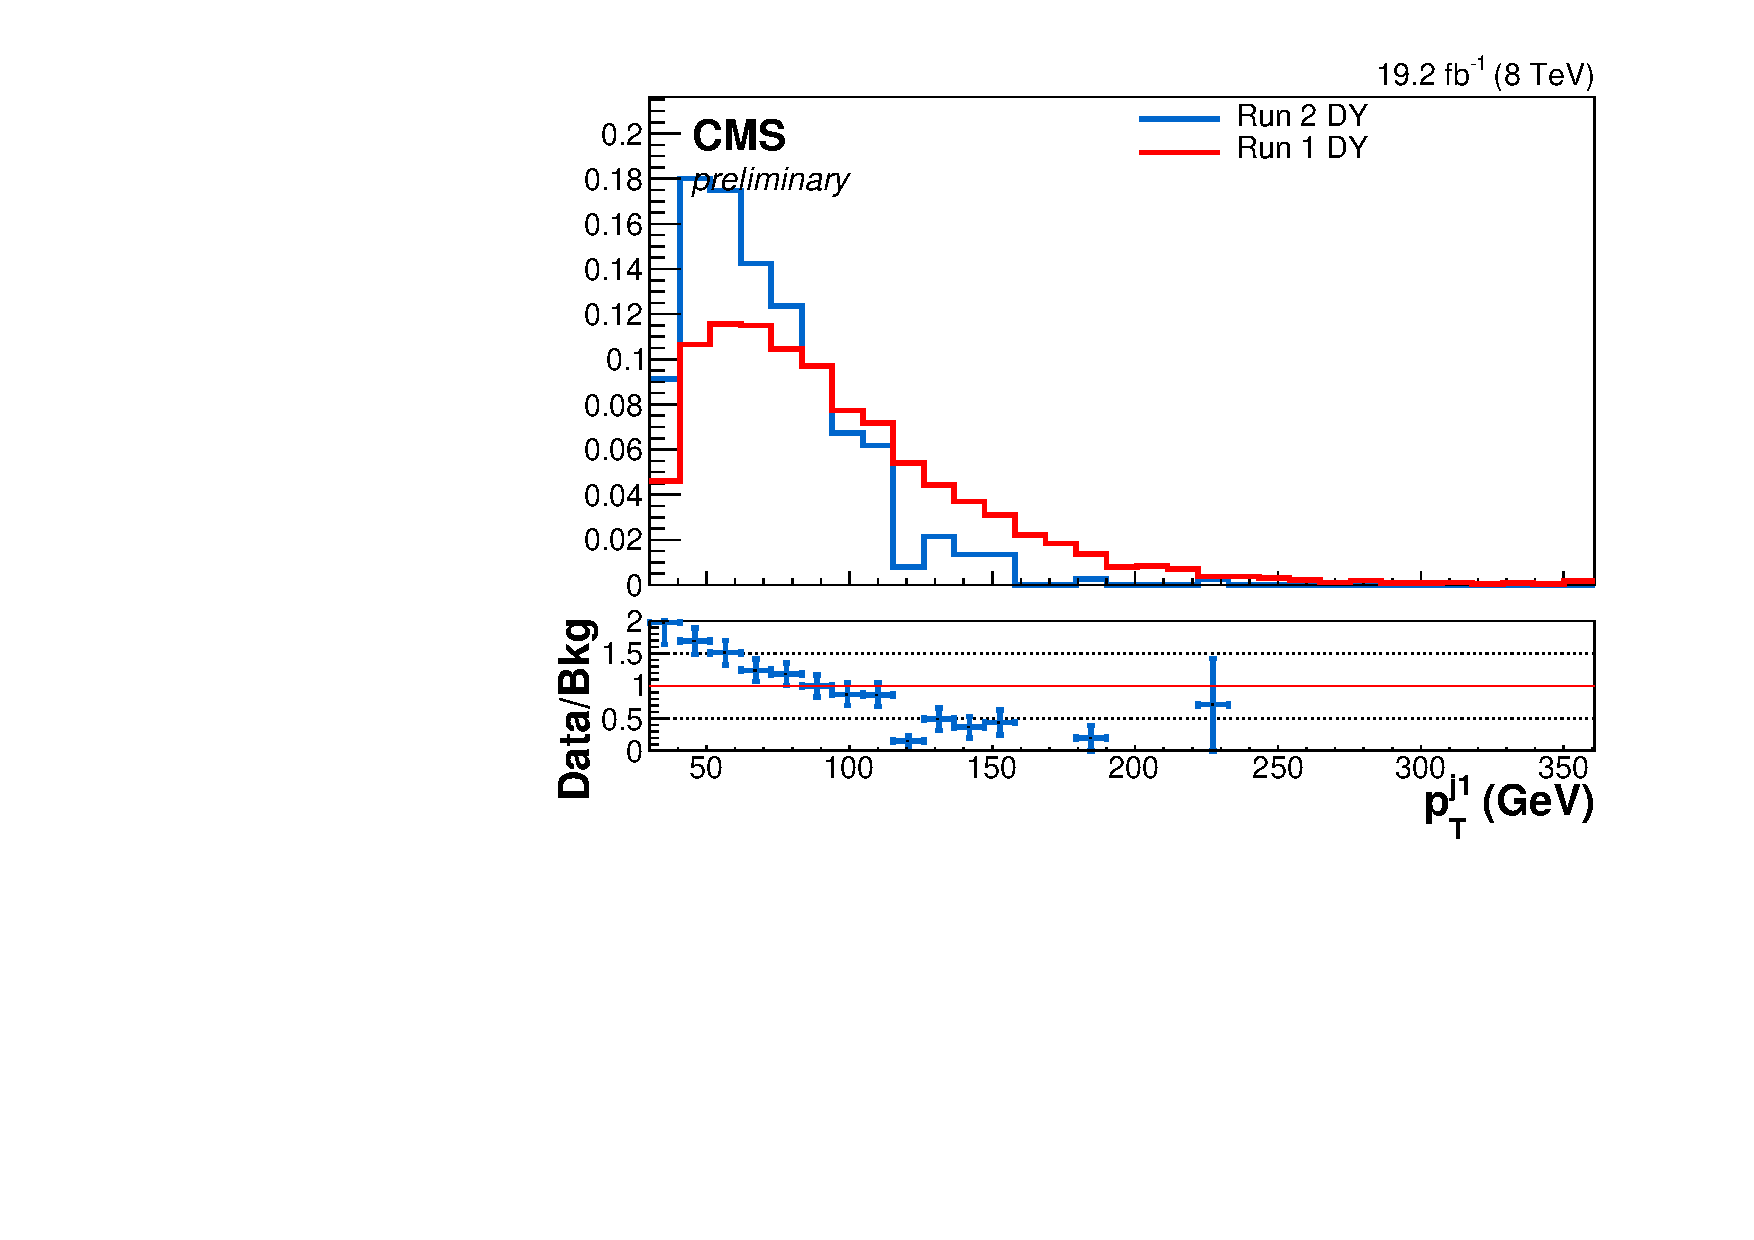
\includegraphics[width=.5\textwidth]{TalkPics/mcstatus080615/output_run1compdynoweight/nunu_norm_jet1_pt.pdf}
  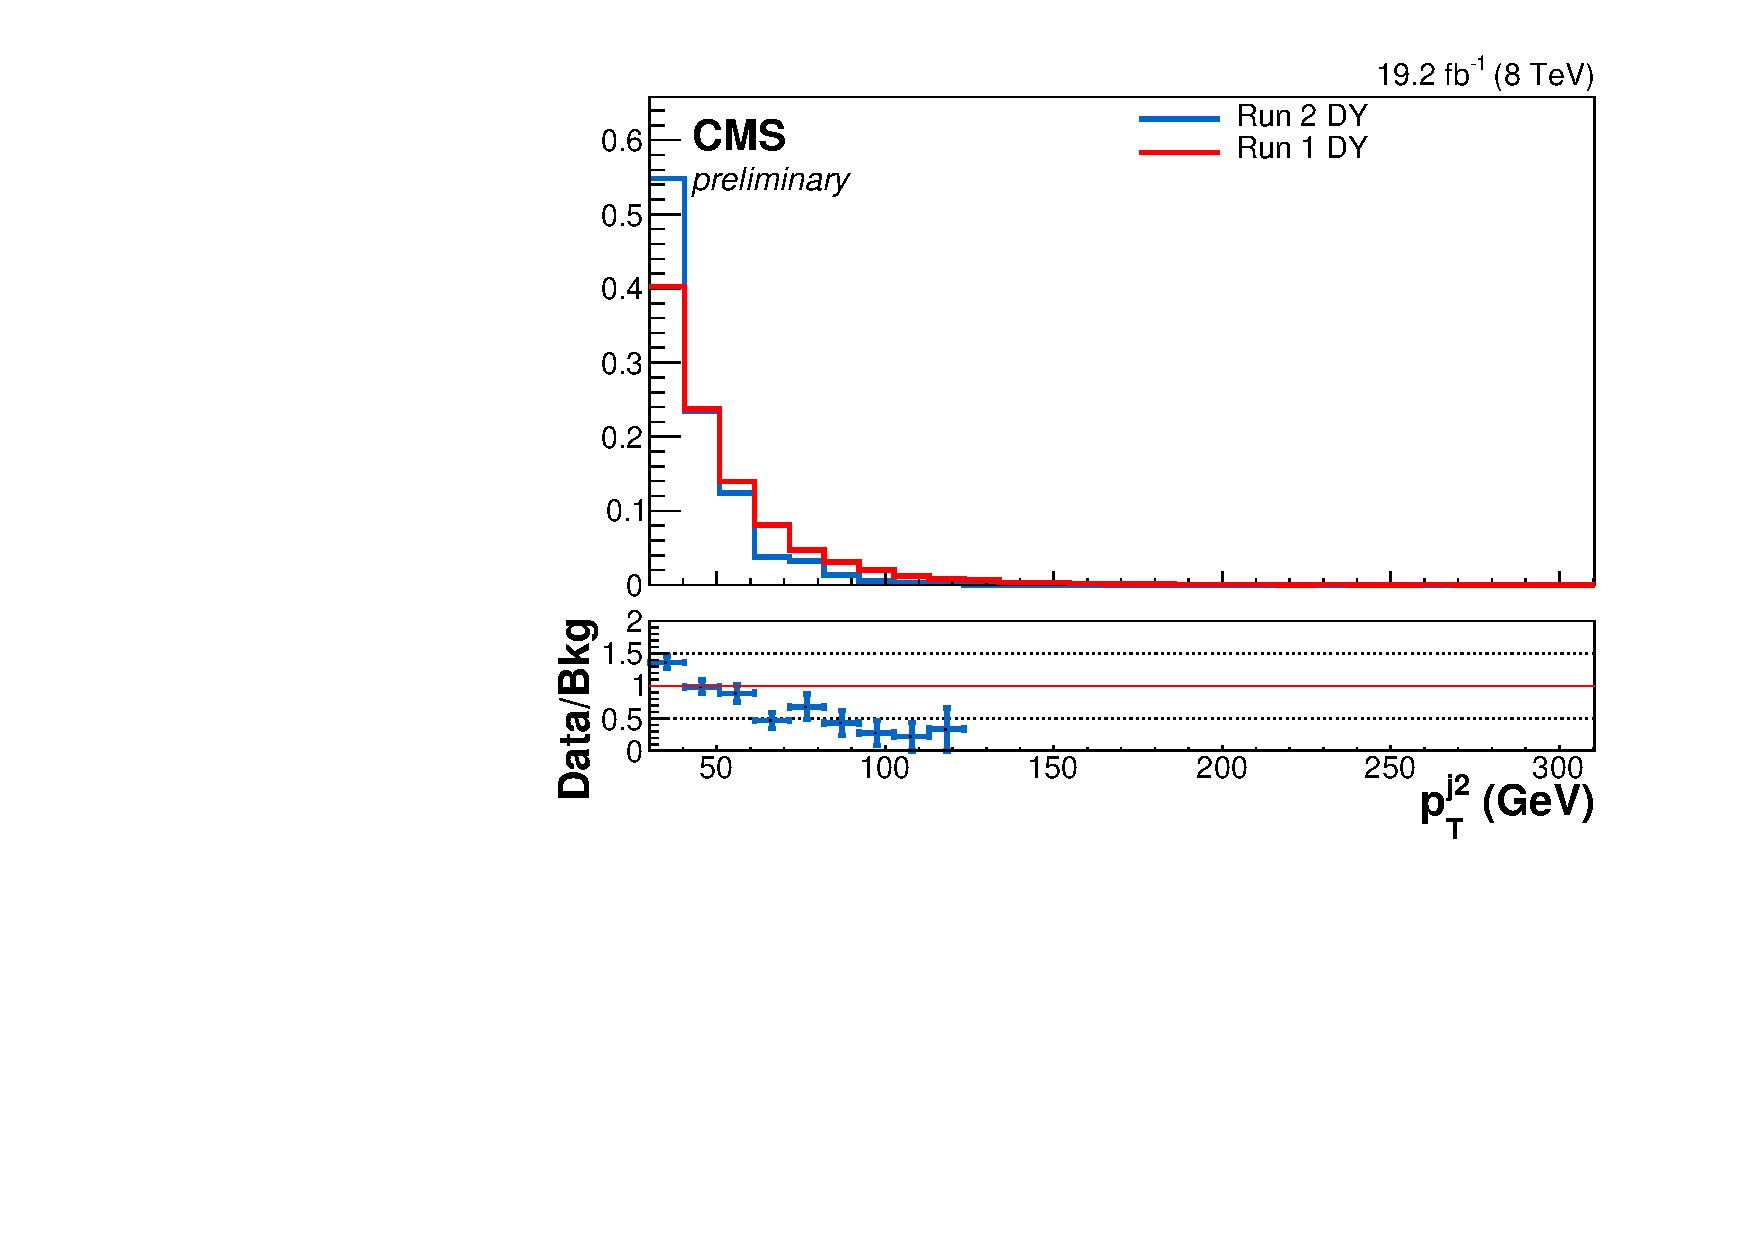
\includegraphics[width=.5\textwidth]{TalkPics/mcstatus080615/output_run1compdynoweight/nunu_norm_jet2_pt.pdf}
  \begin{block}{}
    \begin{itemize}
    \item[-] Low statistics in run 2 MC but appears higher in pt
    \end{itemize}
  \end{block}
\end{frame}

\begin{frame}
  \frametitle{DY Comparison: run 1 vs run 2: Jet $\eta$}
  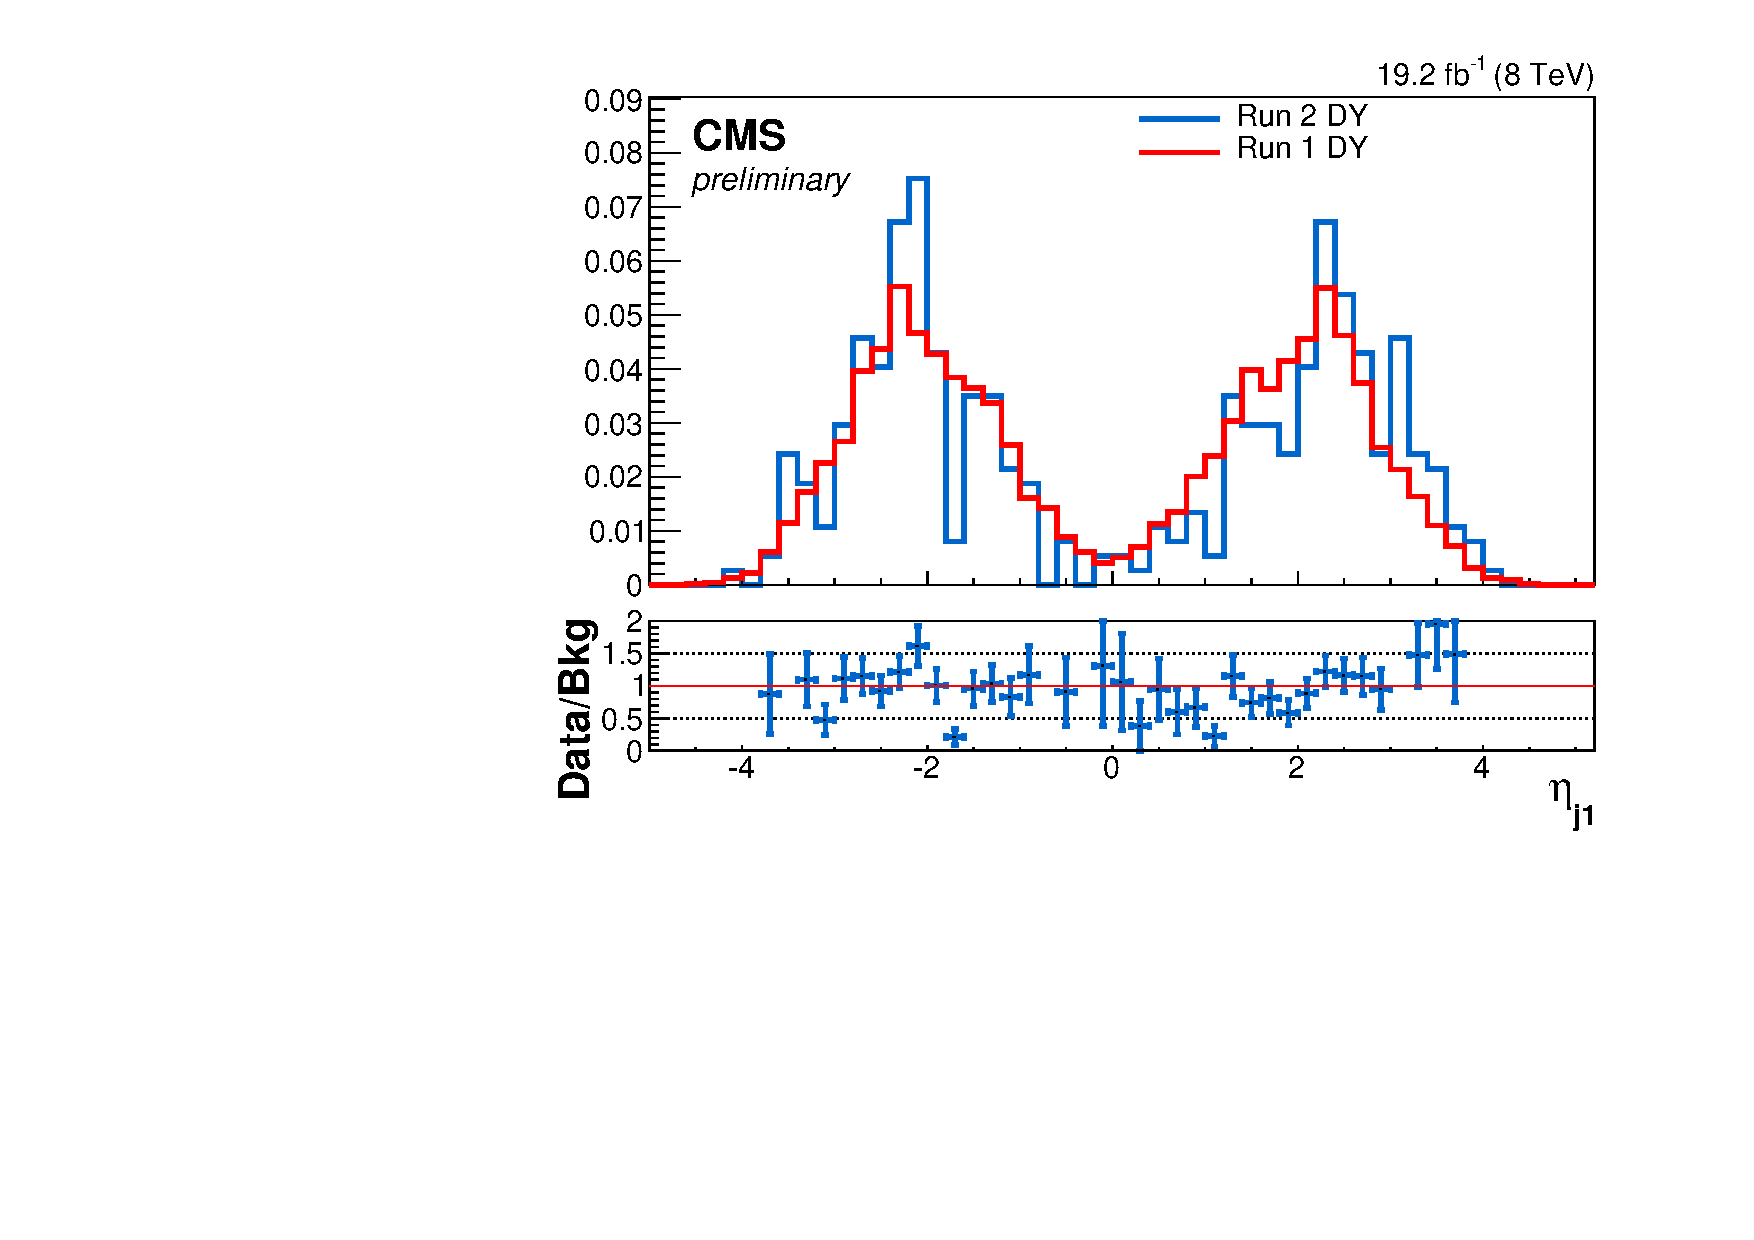
\includegraphics[width=.5\textwidth]{TalkPics/mcstatus080615/output_run1compdynoweight/nunu_norm_jet1_eta.pdf}
  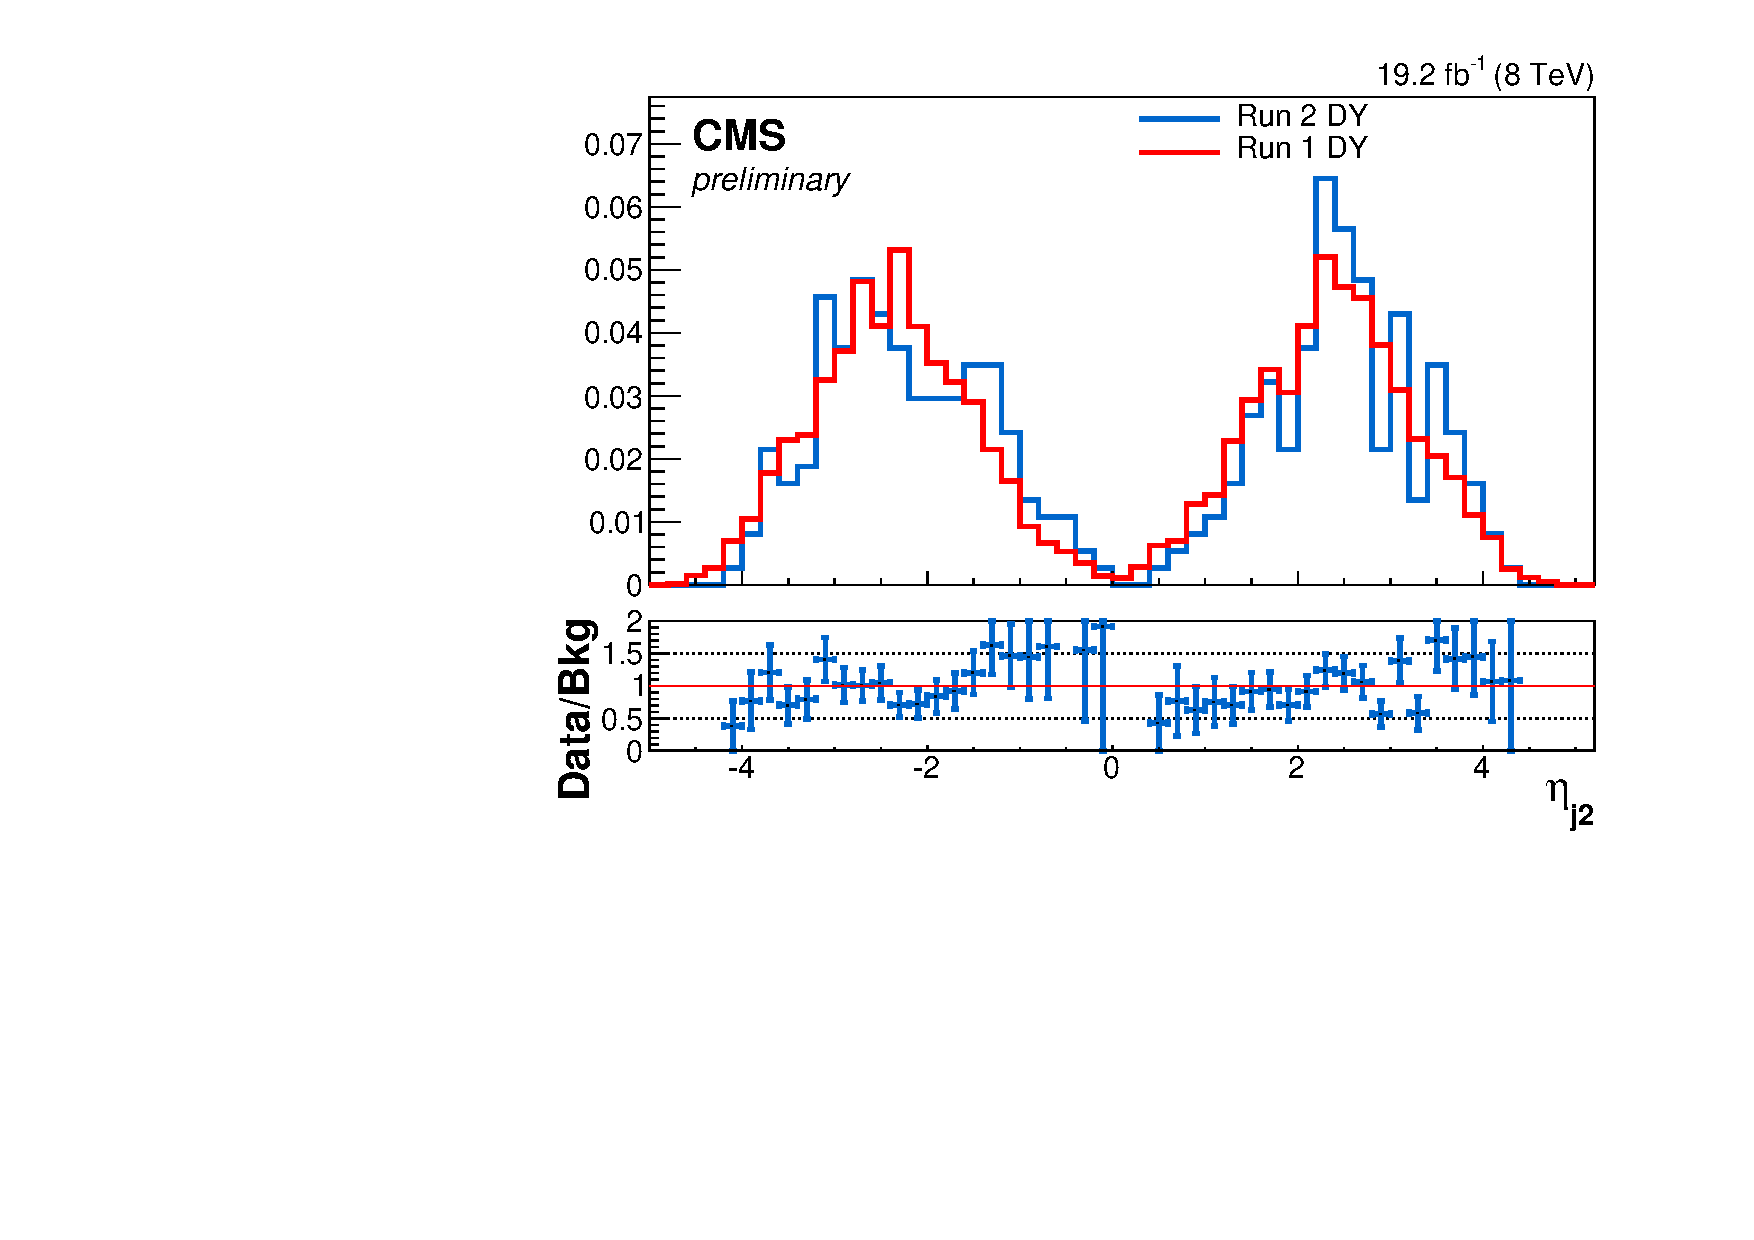
\includegraphics[width=.5\textwidth]{TalkPics/mcstatus080615/output_run1compdynoweight/nunu_norm_jet2_eta.pdf}
  \begin{block}{}
    \begin{itemize}
    \item Ears still apparent
    \end{itemize}
  \end{block}
\end{frame}

\begin{frame}
  \frametitle{DY Comparison: run 1 vs run 2: Jet $\phi$}
  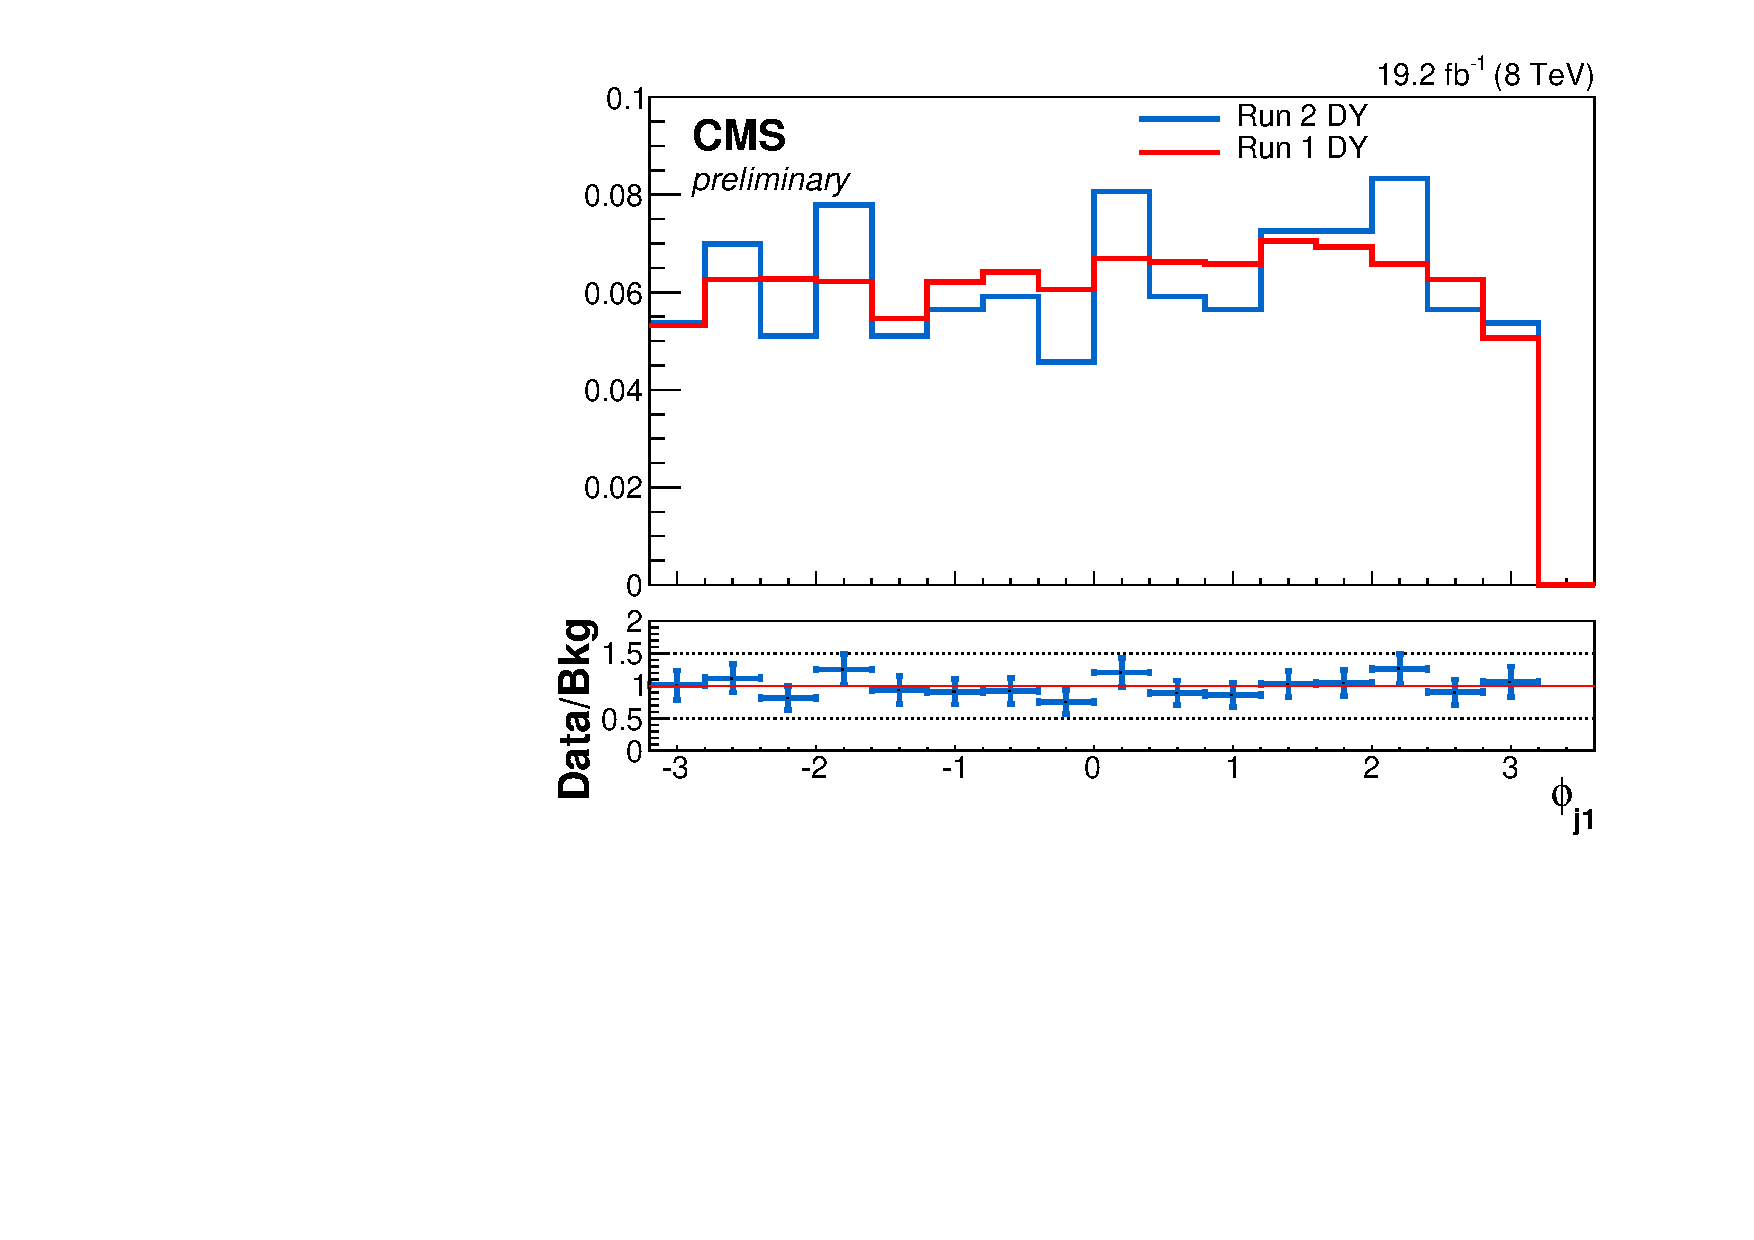
\includegraphics[width=.5\textwidth]{TalkPics/mcstatus080615/output_run1compdynoweight/nunu_norm_jet1_phi.pdf}
  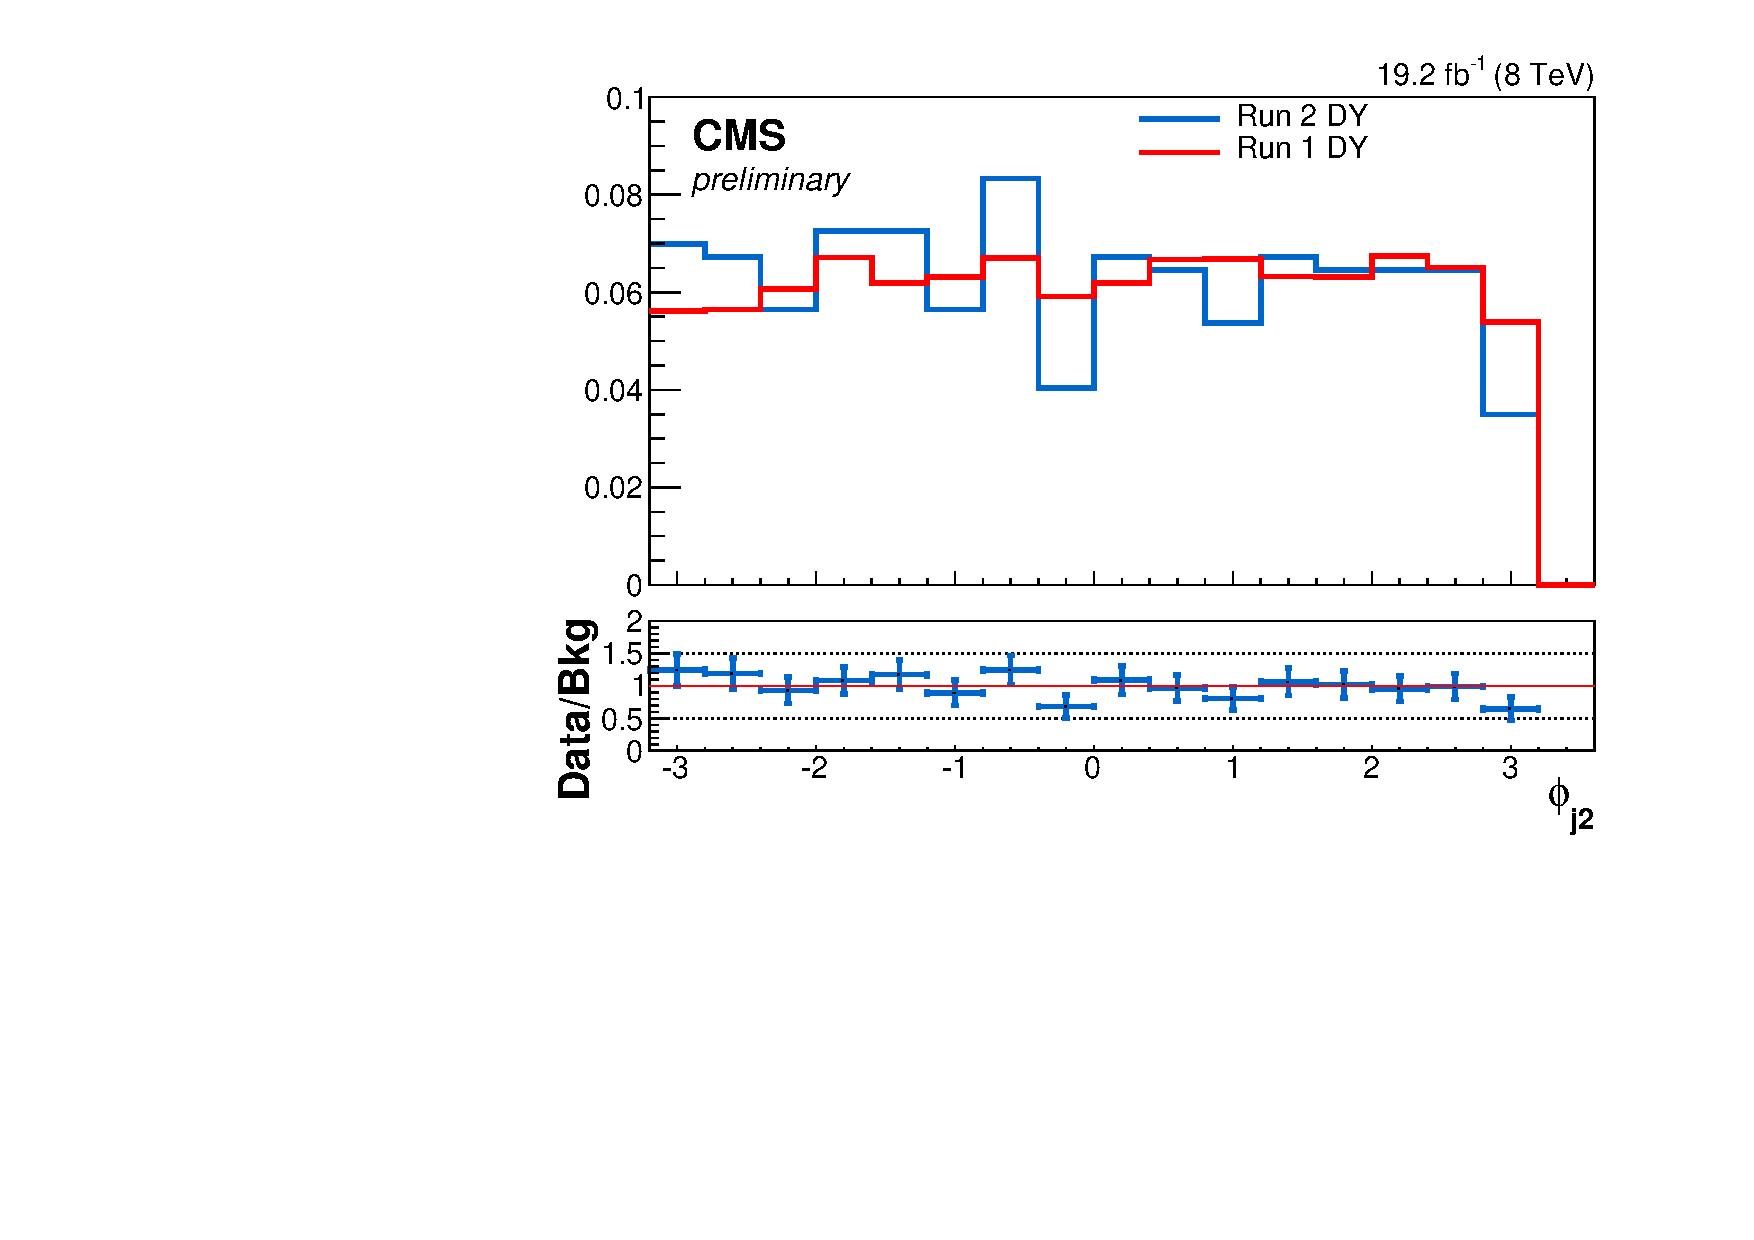
\includegraphics[width=.5\textwidth]{TalkPics/mcstatus080615/output_run1compdynoweight/nunu_norm_jet2_phi.pdf}
  \begin{block}{}
    \begin{itemize}
    \item $\phi$ distributions look similar within stat error
    \end{itemize}
  \end{block}
\end{frame}

\begin{frame}
  \frametitle{DY Comparison: run 1 vs run 2: Met}
  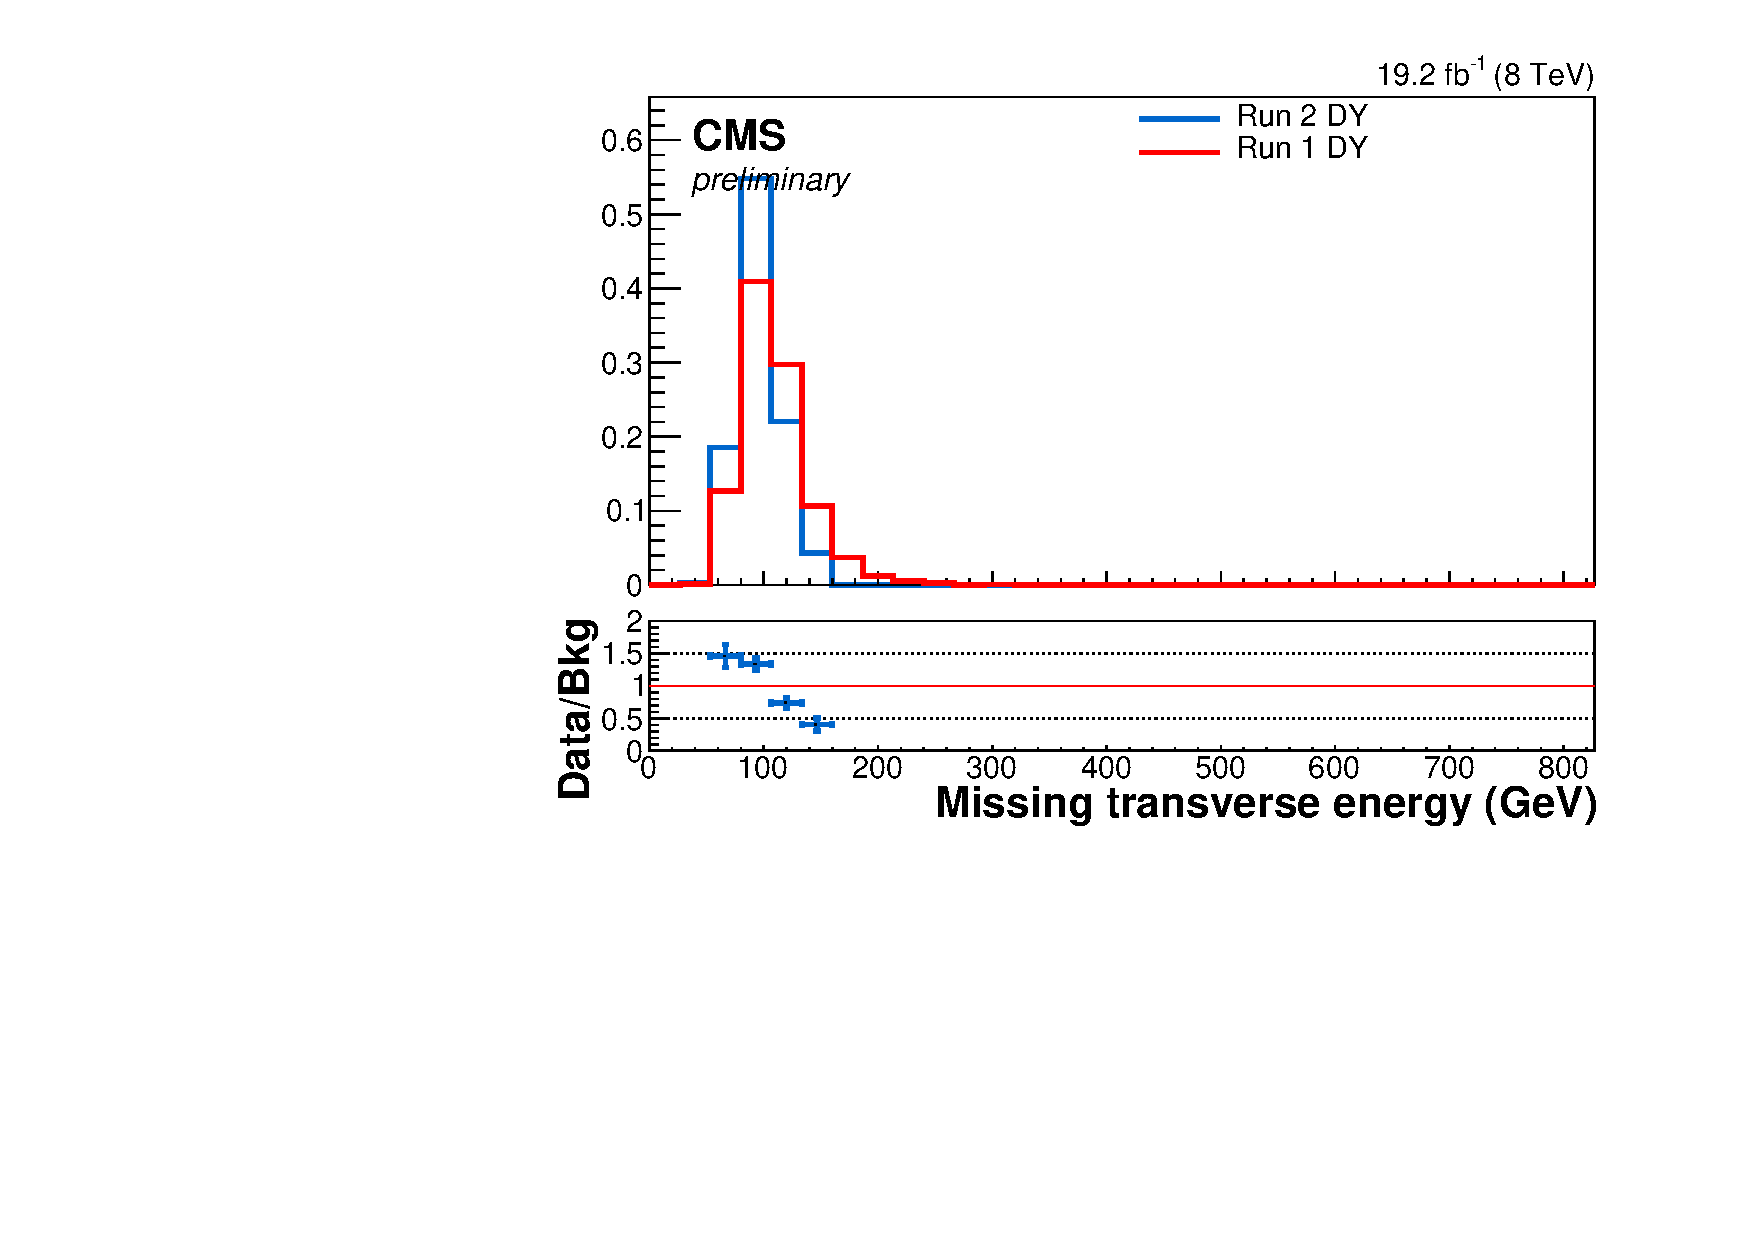
\includegraphics[width=.5\textwidth]{TalkPics/mcstatus080615/output_run1compdynoweight/nunu_norm_metnomuons.pdf}
  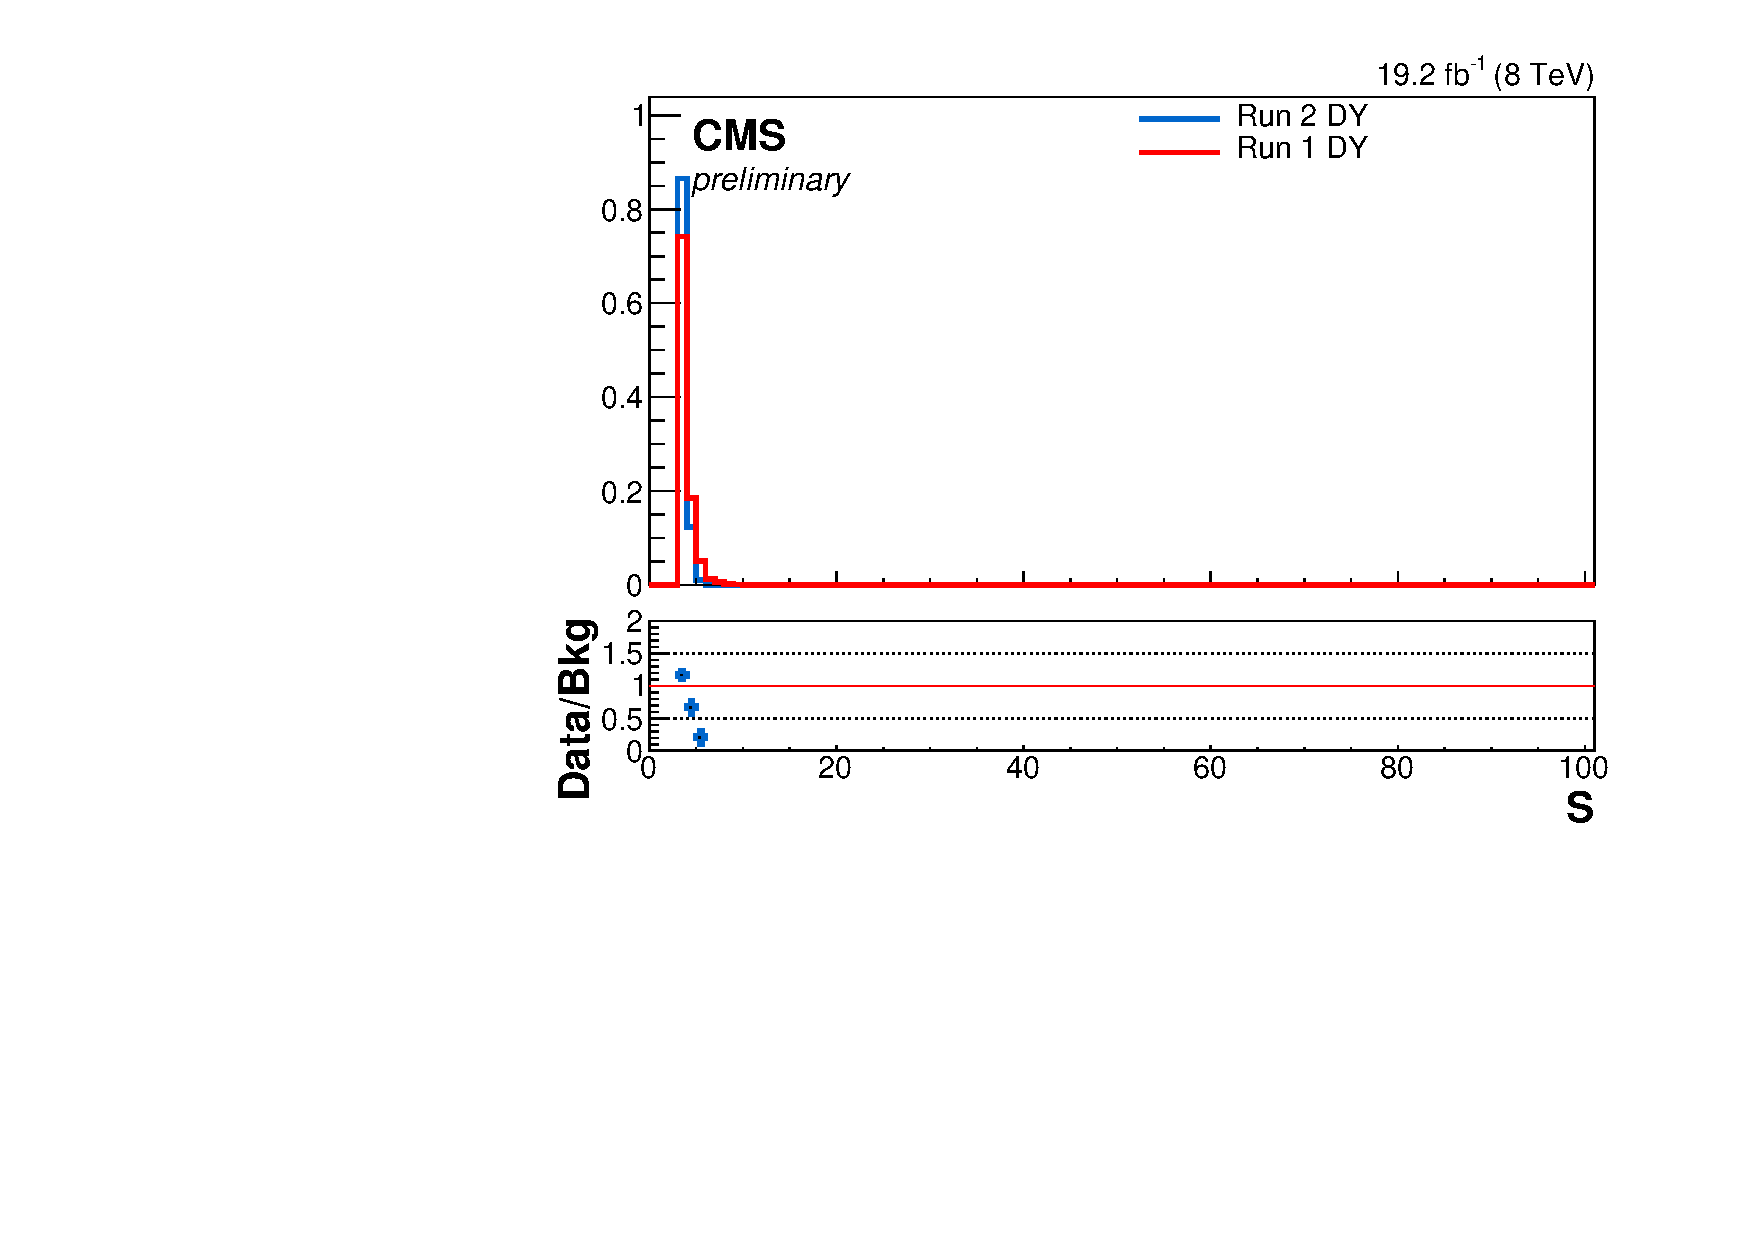
\includegraphics[width=.5\textwidth]{TalkPics/mcstatus080615/output_run1compdynoweight/nunu_norm_metnomu_significance.pdf}
  \begin{block}{}
    \begin{itemize}
    \item Metnomu lower for run 2
    \item Met significance is a different variable in miniAOD to the one we used in run 1
    \end{itemize}
  \end{block}
\end{frame}

\begin{frame}
  \frametitle{DY Comparison: run 1 vs run 2: $\Delta\phi$ variables}
  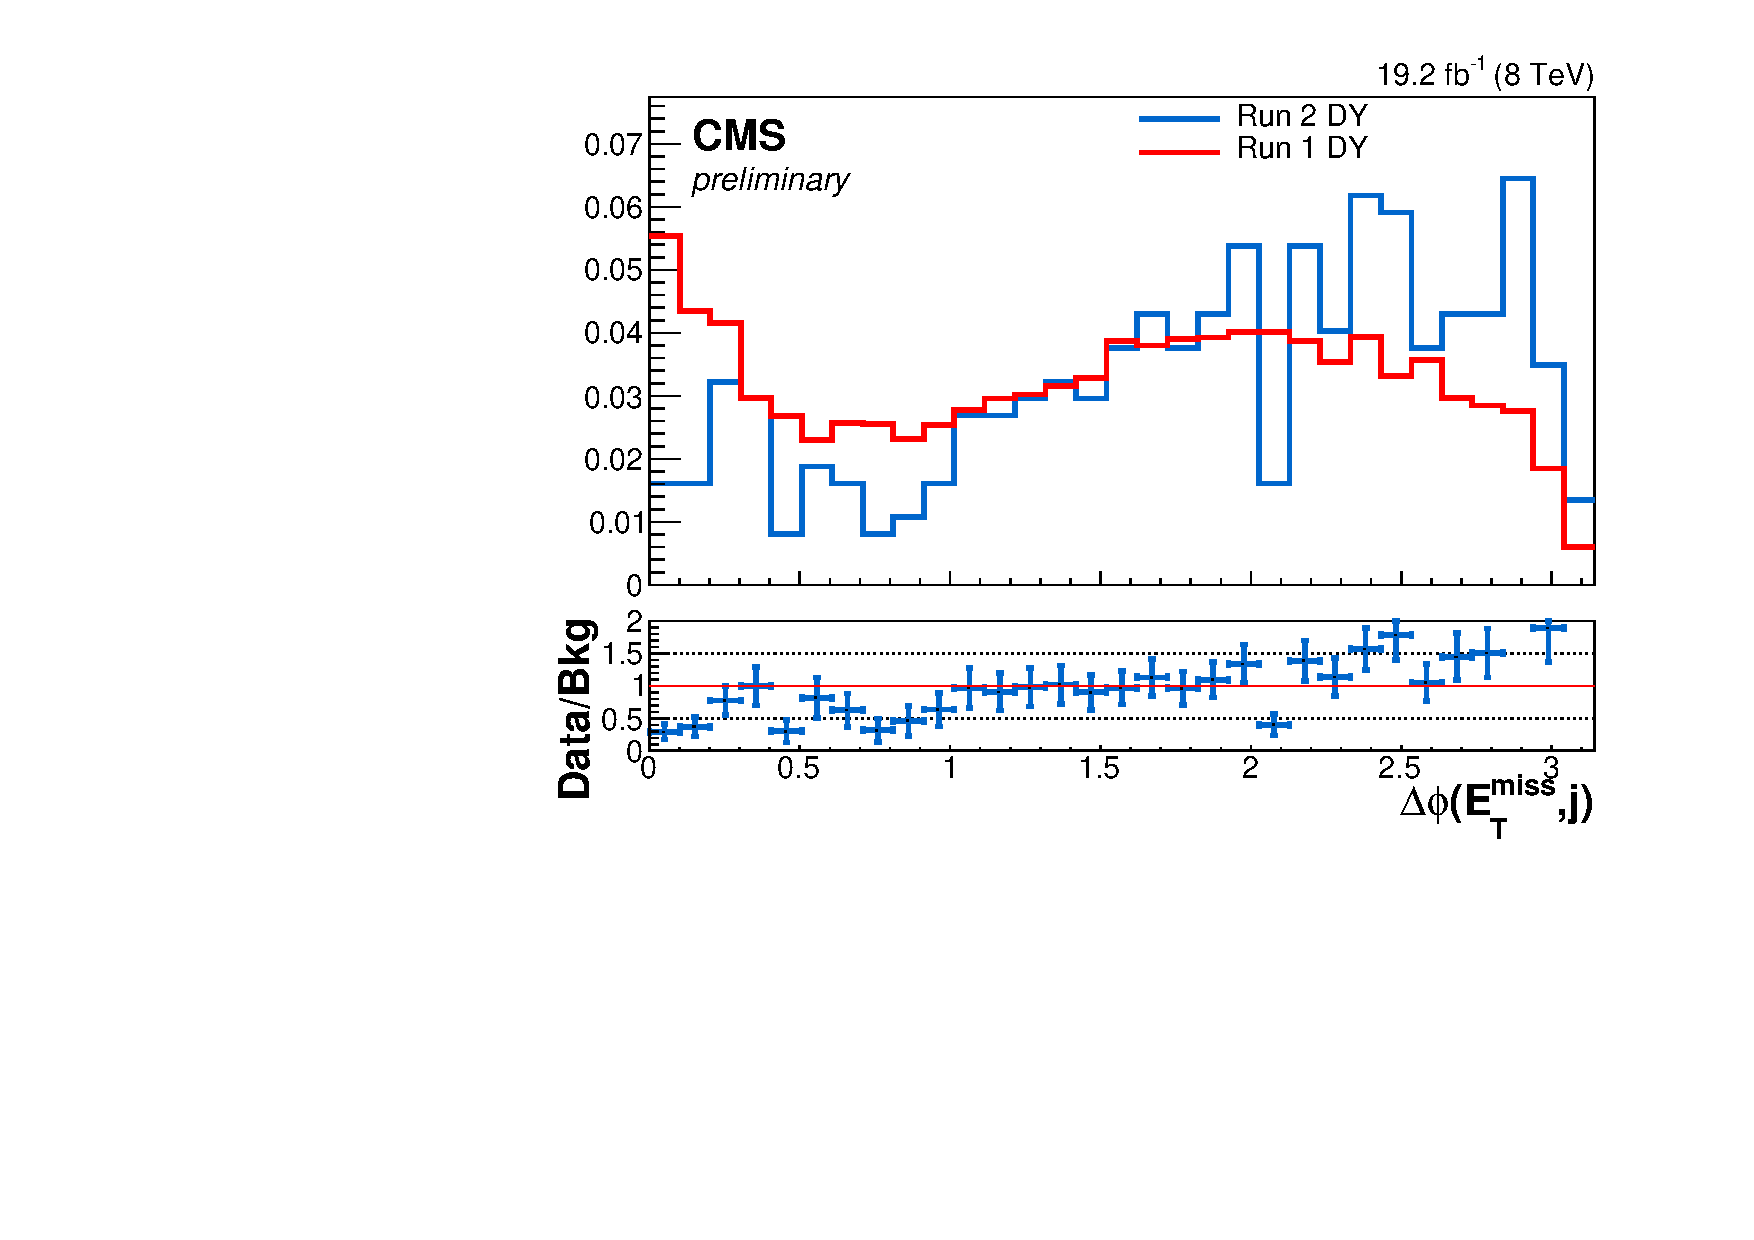
\includegraphics[width=.5\textwidth]{TalkPics/mcstatus080615/output_run1compdynoweight/nunu_norm_alljetsmetnomu_mindphi.pdf}
  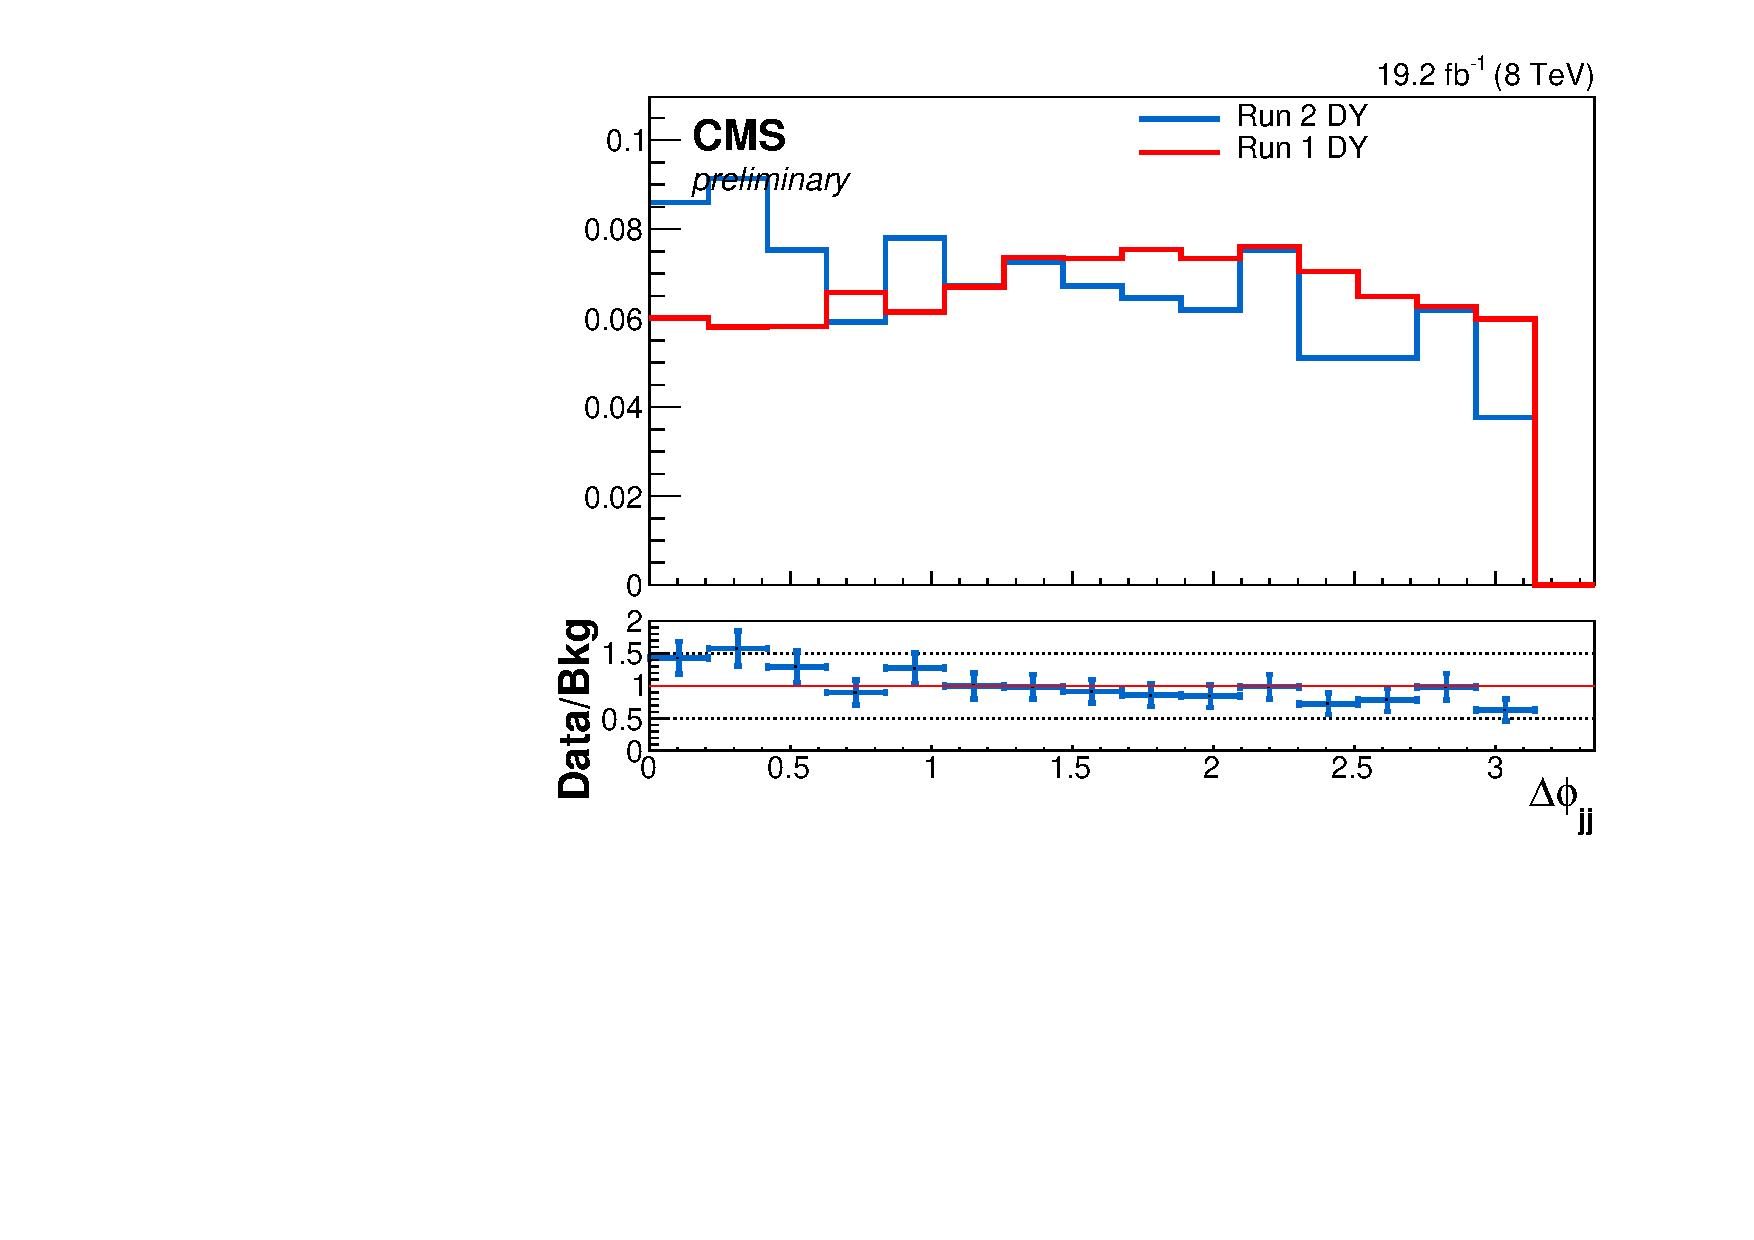
\includegraphics[width=.5\textwidth]{TalkPics/mcstatus080615/output_run1compdynoweight/nunu_norm_dijet_dphi.pdf}
  \begin{block}{}
    \begin{itemize}
    \item Limited by low stats
    \end{itemize}
  \end{block}
\end{frame}

\begin{frame}
  \frametitle{DY Comparison: run 1 vs run 2: dijet variables}
  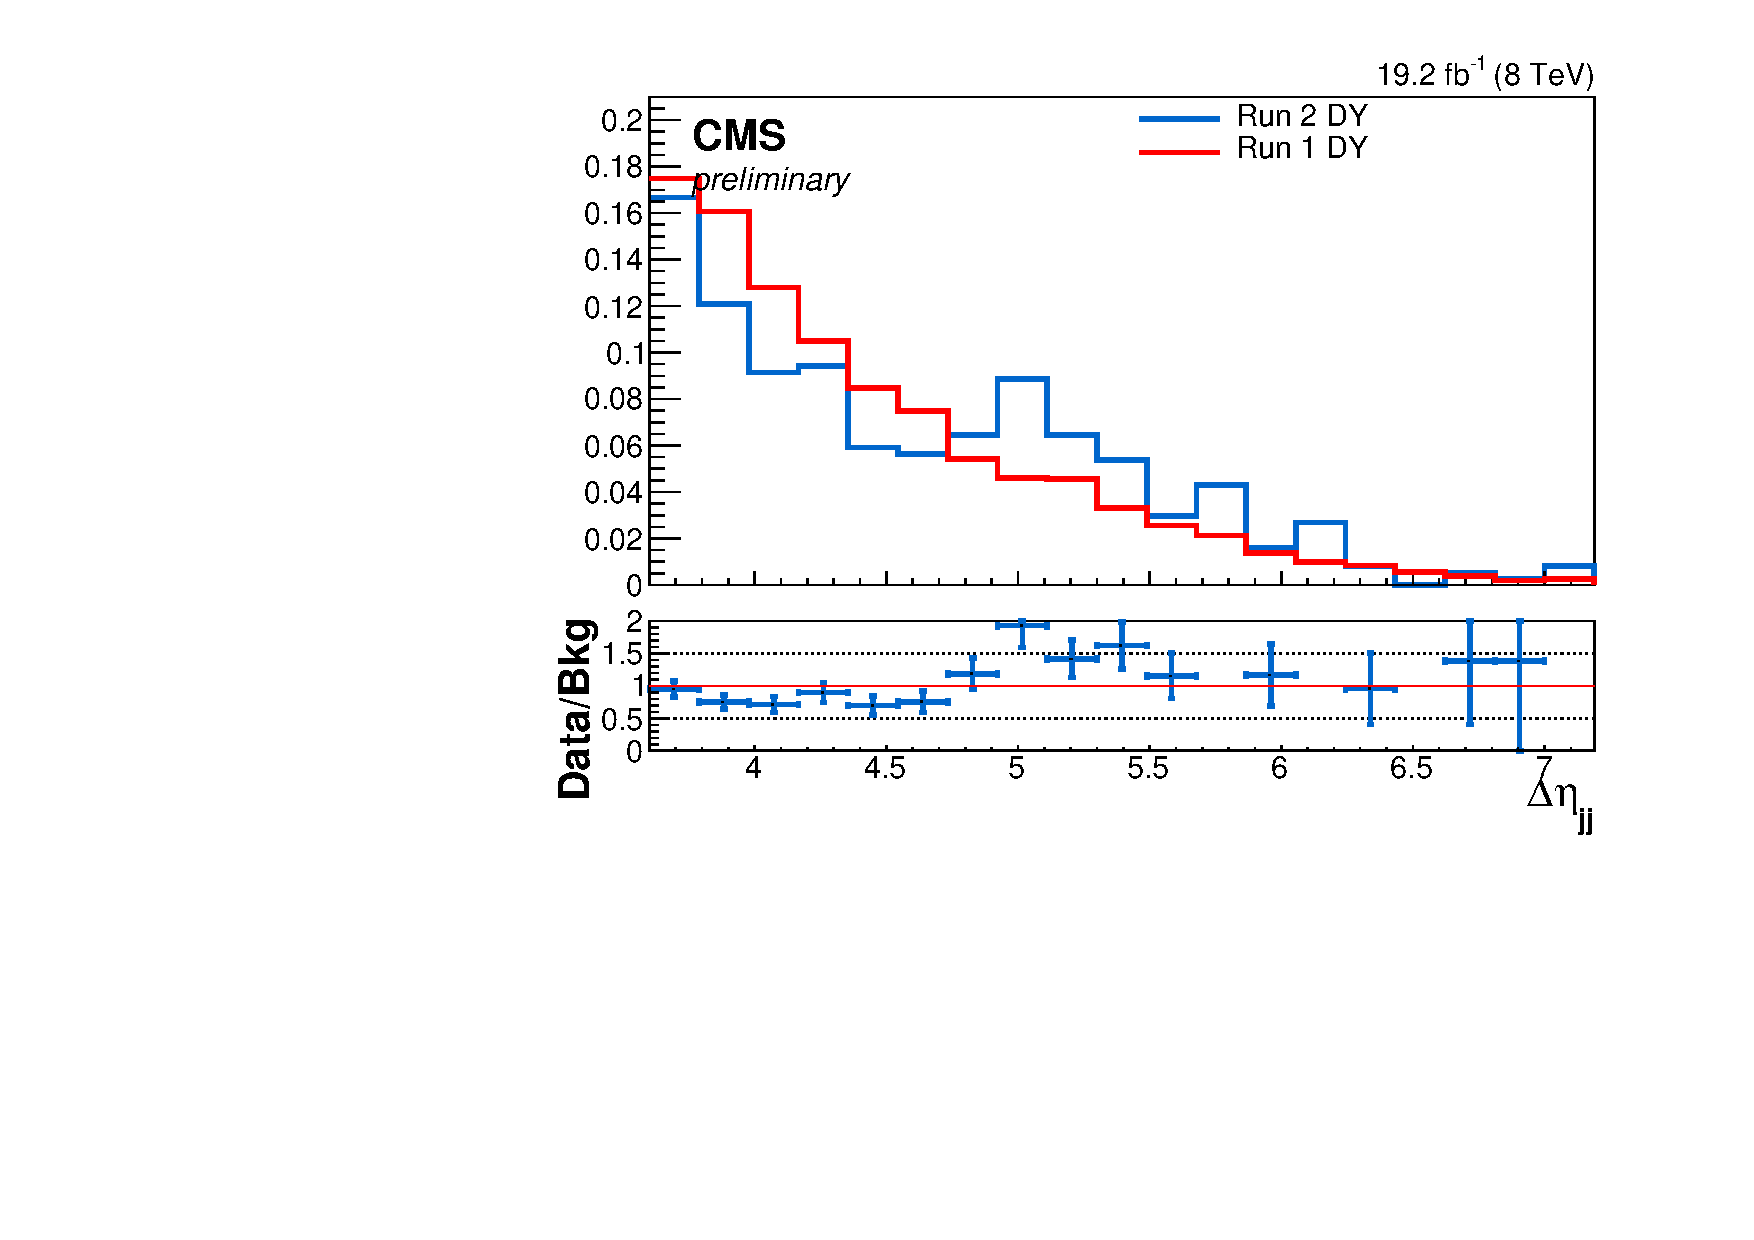
\includegraphics[width=.5\textwidth]{TalkPics/mcstatus080615/output_run1compdynoweight/nunu_norm_dijet_deta.pdf}
  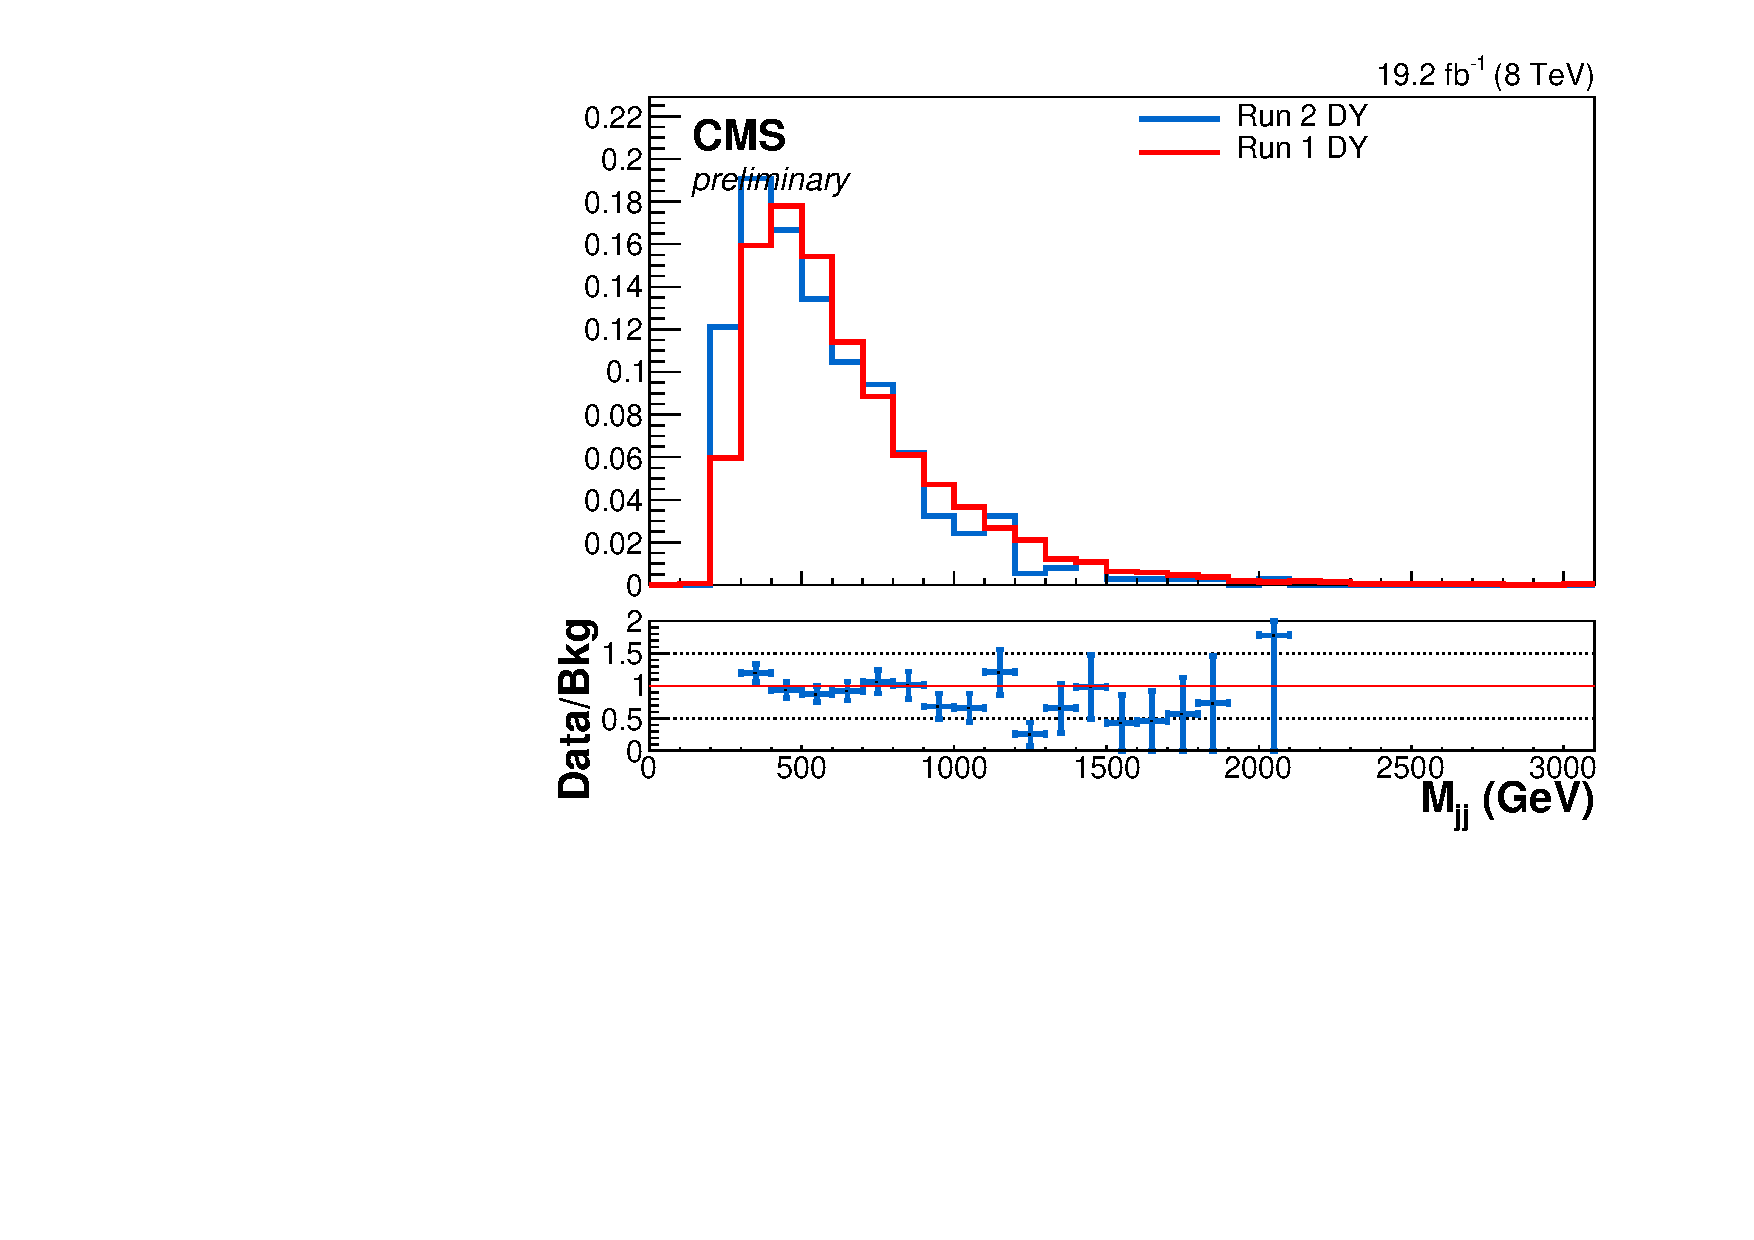
\includegraphics[width=.5\textwidth]{TalkPics/mcstatus080615/output_run1compdynoweight/nunu_norm_dijet_M.pdf}
   \begin{block}{}
     \begin{itemize}
     \item Limited by low stats
     \end{itemize}
   \end{block}
\end{frame}

\begin{frame}
  \frametitle{DY Comparison: run 1 vs run 2: N jets}
  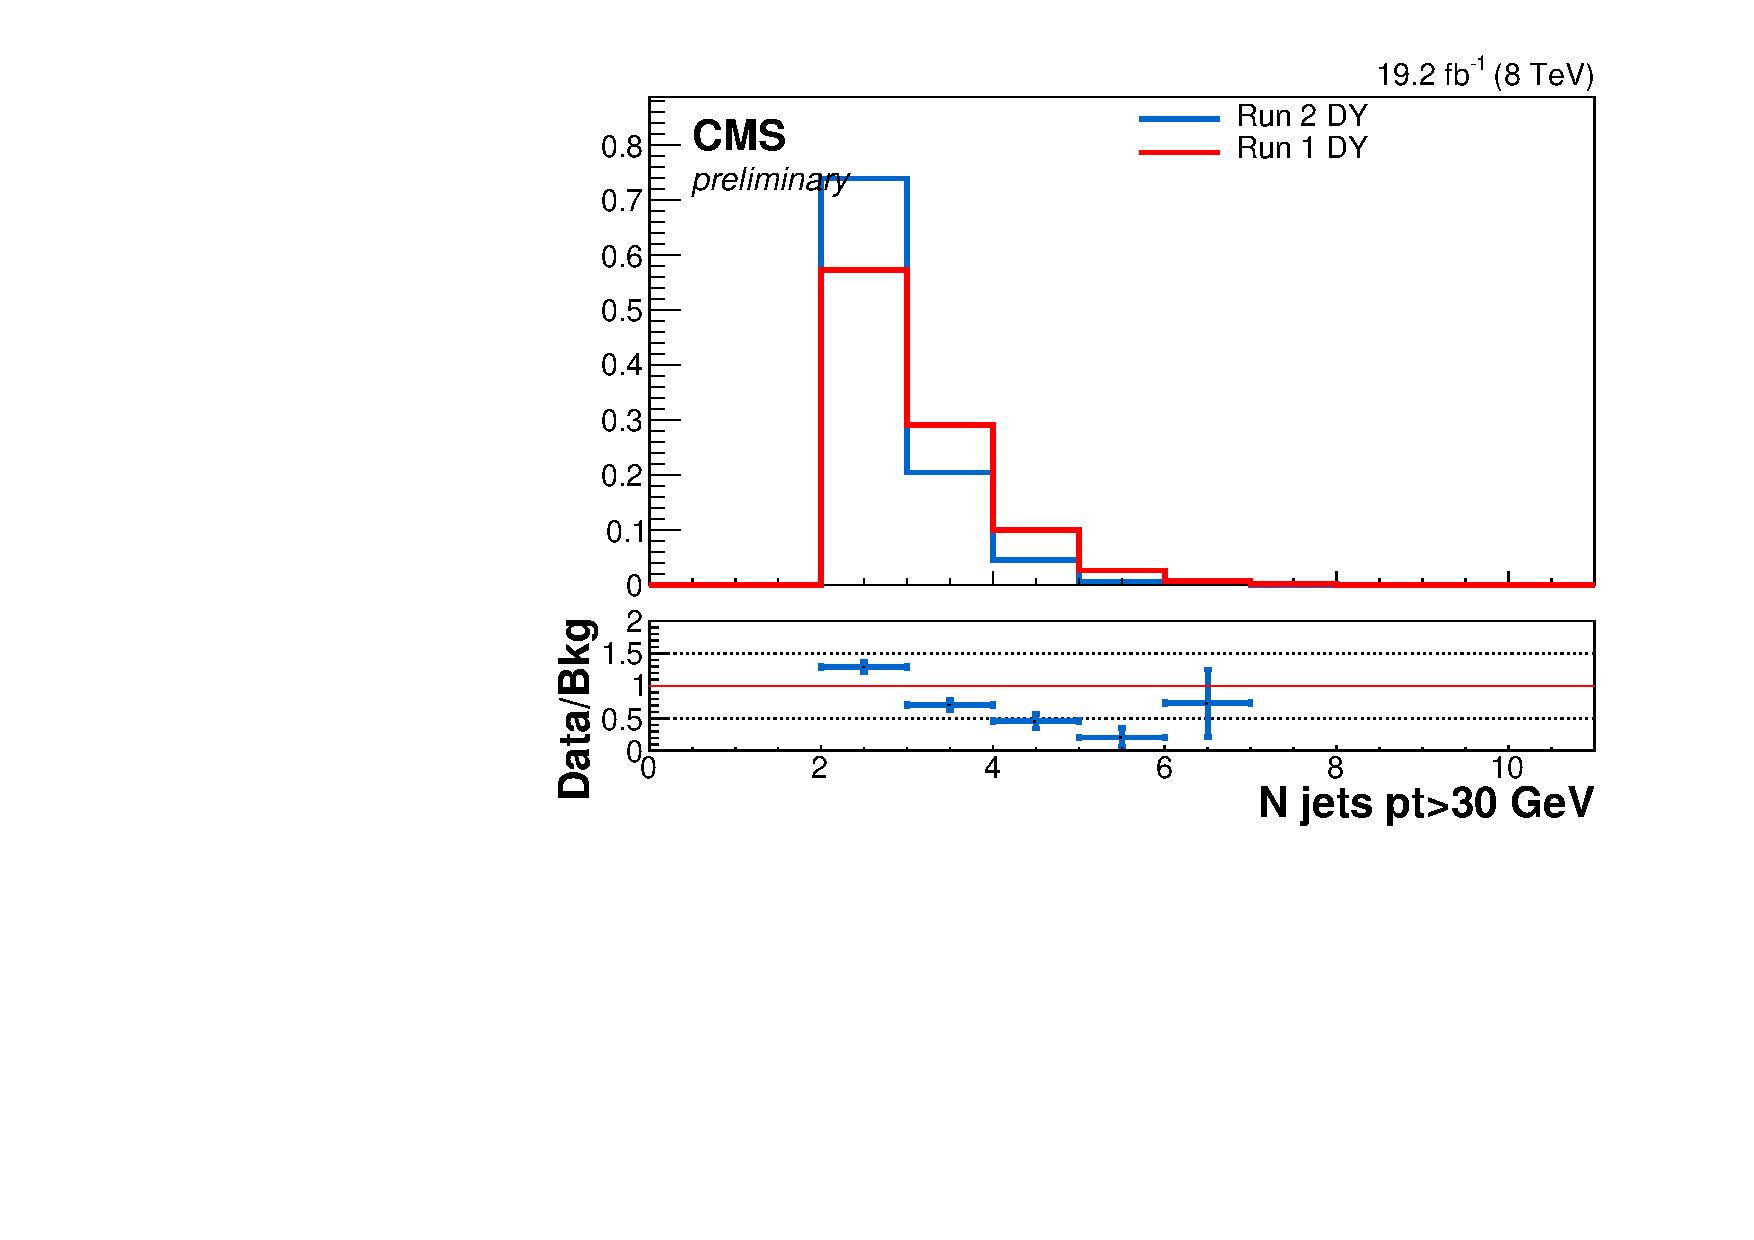
\includegraphics[width=.5\textwidth]{TalkPics/mcstatus080615/output_run1compdynoweight/nunu_norm_n_jets_30.pdf}
  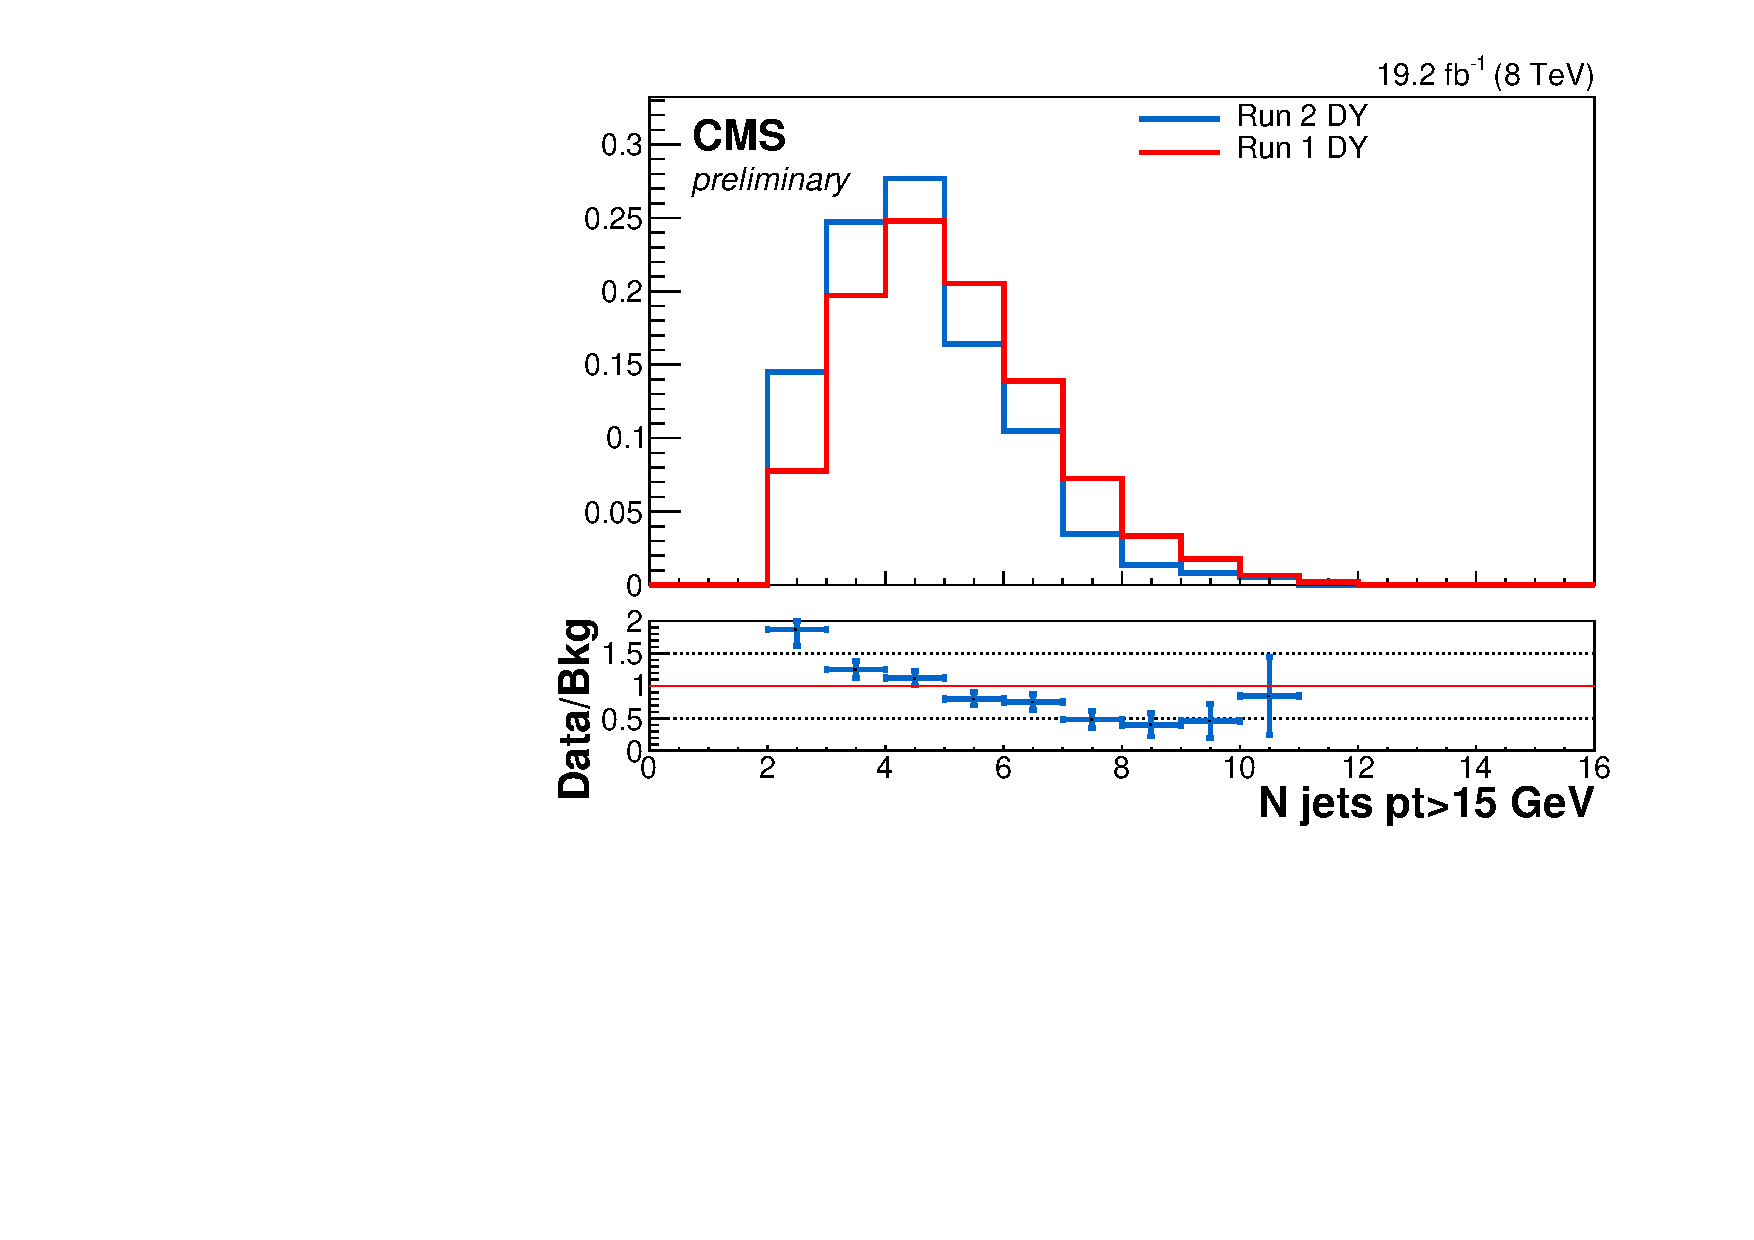
\includegraphics[width=.5\textwidth]{TalkPics/mcstatus080615/output_run1compdynoweight/nunu_norm_n_jets_15.pdf}
\end{frame}

\begin{frame}
  \frametitle{W MC: replacing status 3}
  \begin{block}{}
    \begin{itemize}
    \item According to \href{http://home.thep.lu.se/~torbjorn/pythia81html/ParticleProperties.html}{pythia 8 documentation} status 21-29 replaces status 3
    \item Check for status 3 lepton $\rightarrow$ check for status 21-29 lepton
    \end{itemize}
    \begin{center}
      \begin{tabular}{|l|c|c|}
        \hline
        Channel & Inclusive & Split \\
        \hline
        enu & N/A & 1880521 \\
        munu & N/A & 1772078 \\
        taunu & N/A & 738104 \\
        \hline
        total & 10017462 & 4390703 \\
        \hline
      \end{tabular}
    \end{center}
      \begin{itemize}
    \item Over half of the events are missing
    \end{itemize}
  \end{block}
\end{frame}

\begin{frame}
  \frametitle{W MC: replacing status 3}
  \begin{block}{}
    \begin{itemize}
    \item Check lists of gen particles in events
    \item All events have a status 22 W as expected:
    \item[-] status 22 means hard scatter incoming
    \item Naively expect one status 23 lepton:
    \item[-] status 23 means hard scatter outgoing
    \item All events have at least one lepton but often not status 23
    \item From GEN hypernews it appears status 23 particles with no FSR replaced with status 1
    \item Often many status 1 and 2 leptons need to find one from W
    \end{itemize}
  \end{block}
\end{frame}

\begin{frame}
  \frametitle{W MC: replacing status 3}
  \begin{block}{New strategy}
    \begin{itemize}
    \item Use list of W daughters to find lepton flavour
    \item If a $\tau$ is found check its daughters to determine $\tau$ decay
    \item[-] $\tau$ often radiates, need to check recursively until a decay is found
    \end{itemize}
  \end{block}
  \begin{block}{}
    \begin{itemize}
    \item This correctly classifies most events, still trying to find out what happens to the others
    \end{itemize}
  \end{block}
\end{frame}



\begin{frame}
  \frametitle{Higgs Portal DM interpretation - update}
  \vspace{-.3cm}
  \begin{block}{}
    \begin{itemize}
    \item Vector line removed after discussion last week
    \item[-] Bjoern asking theorists if there are other models with $\mathcal{B}(H\rightarrow inv)$ expressions
    \item Left plot has three values of fN as in paper
    \item Right plot is prompt (dashed) vs parked (solid)
    \end{itemize}
  \end{block}
  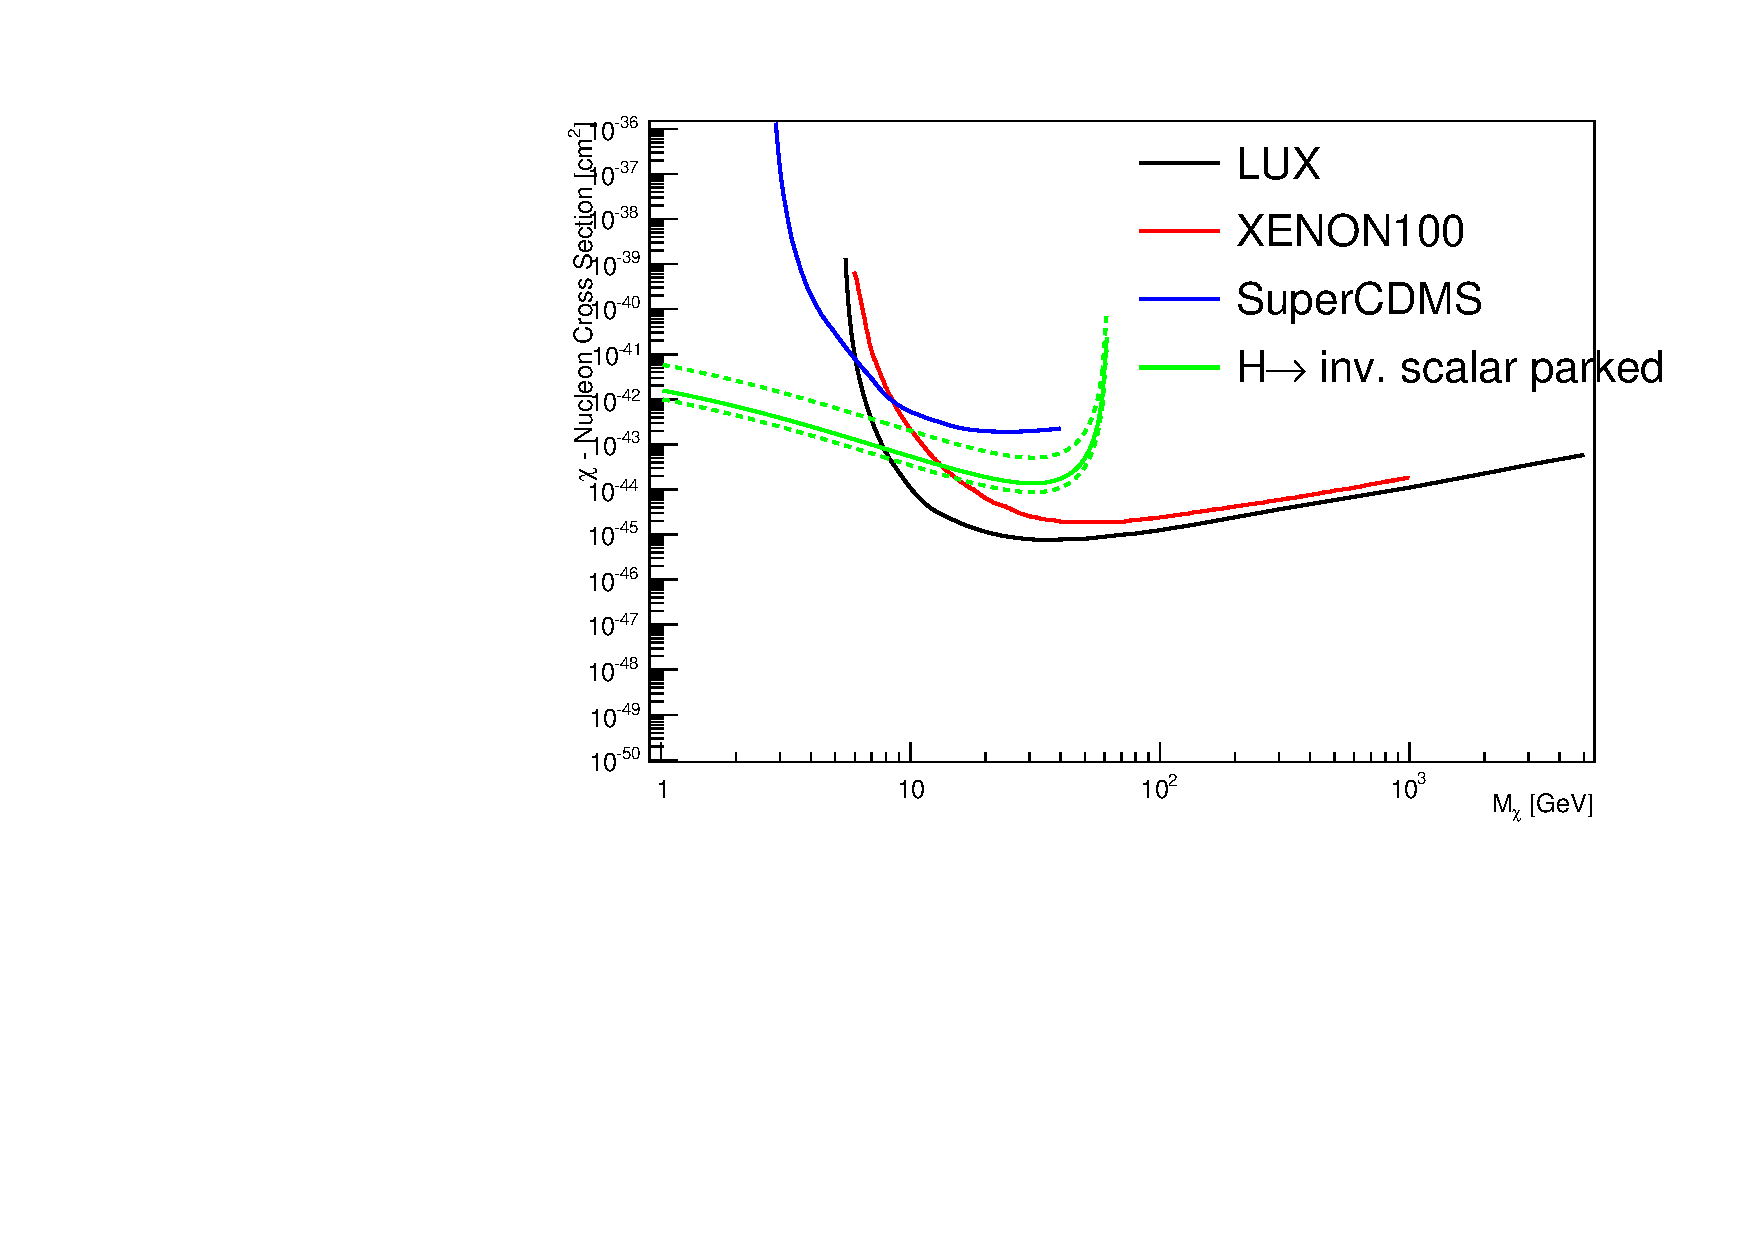
\includegraphics[width=.5\textwidth]{TalkPics/mcstatus080615/DMplot.pdf}
  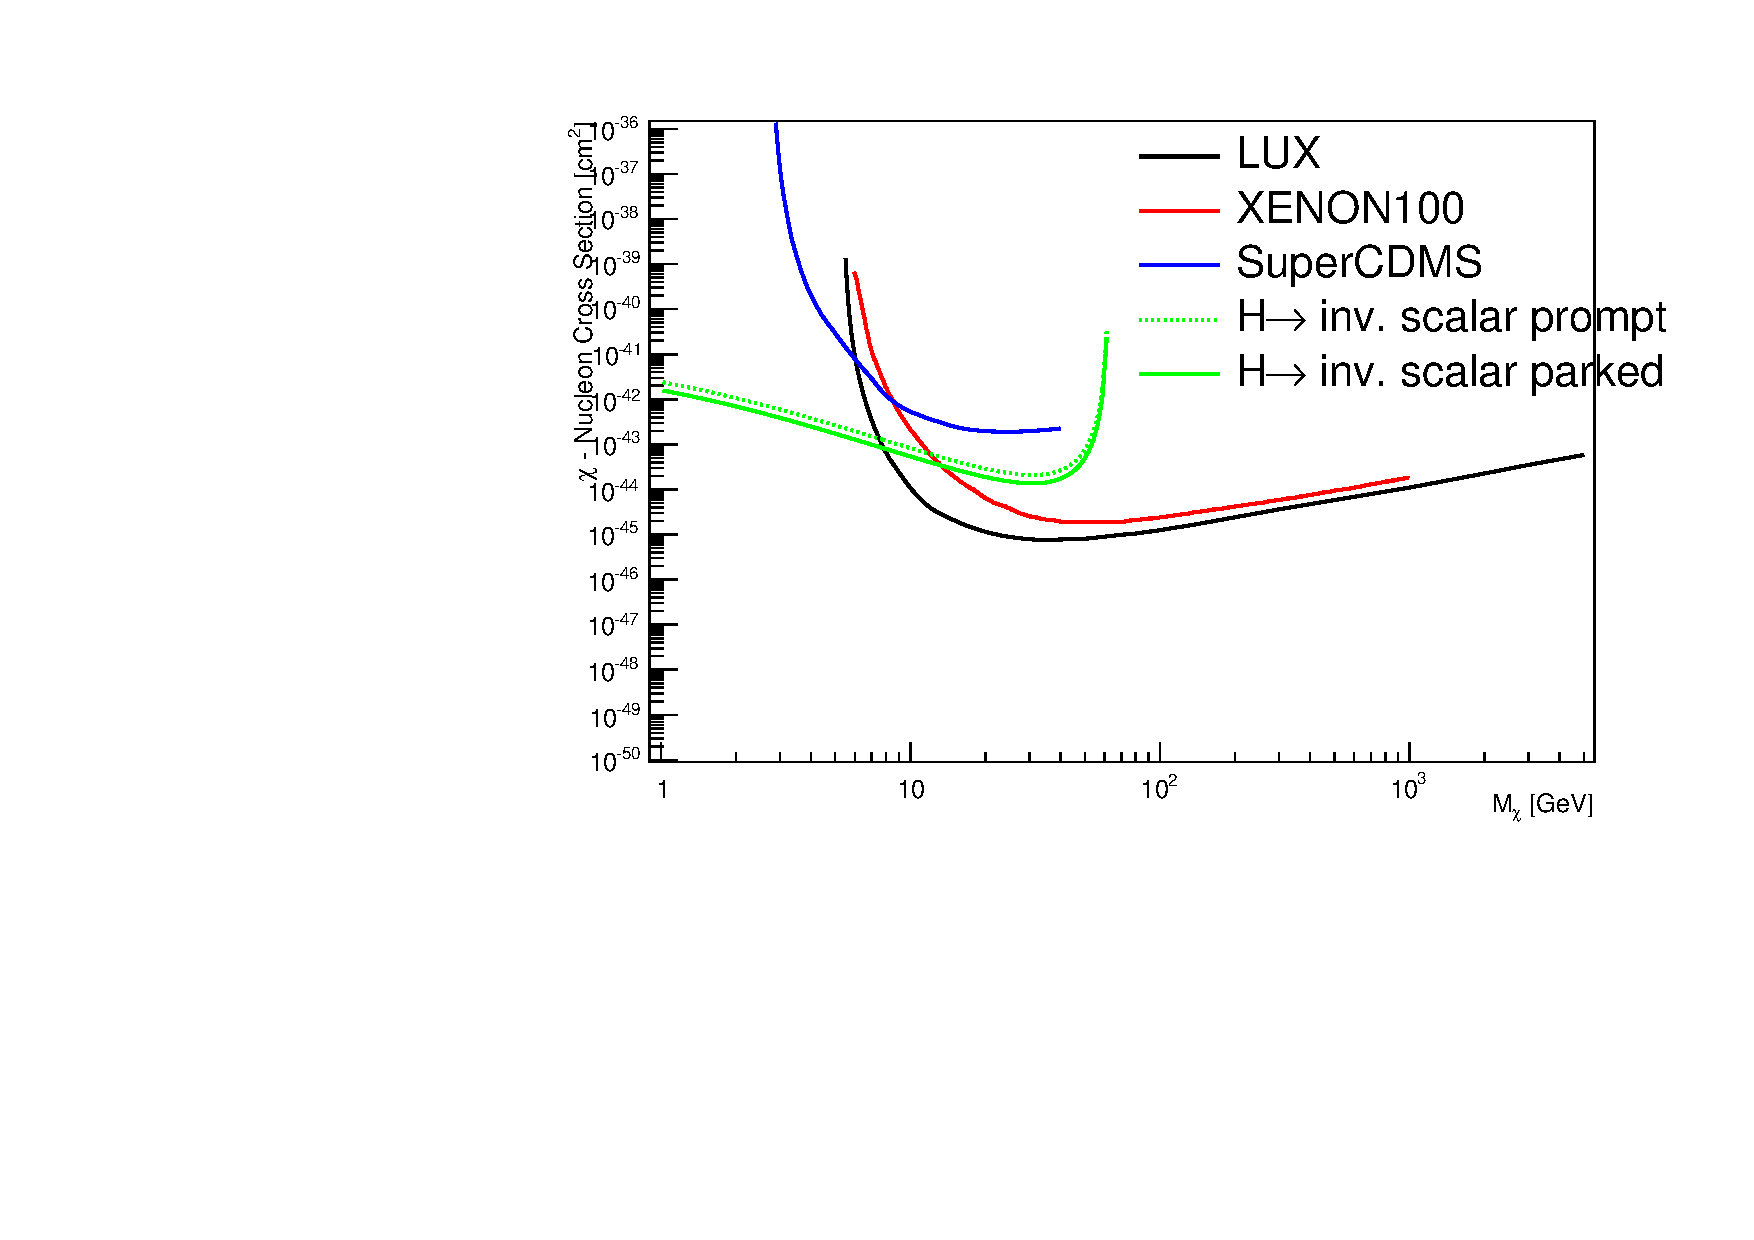
\includegraphics[width=.5\textwidth]{TalkPics/mcstatus080615/DMplotpromptvsparked.pdf}
\end{frame}

\begin{frame}
  \label{lastframe}
  \begin{block}{Summary}
    \begin{itemize}
    \item W and Z MC processed
    \item Z control plots available
    \item W generator level information studies are ongoing
    \item Parked interpretation work is ongoing
    \end{itemize}
  \end{block}
\end{frame}

\begin{frame}
  \frametitle{Backup}
\end{frame}

\end{fmffile}
\end{document}
